% !TeX root = main.tex

\documentclass[10pt,aspectratio=169,dvipsnames]{beamer} % sets document type, default font size, slide aspect ratio, and loads color names
\usetheme[color/block=transparent]{metropolis} % sets the theme of the document

\usepackage[absolute,overlay]{textpos} % allows absolute positioning of text
\usepackage{booktabs} % enhances quality of tables
\usepackage[utf8]{inputenc} % allows input encoding in UTF-8
\usepackage{tikz} % used for creating vector graphics
\usetikzlibrary{arrows.meta} % loads additional arrow types
\usepackage[europeanresistors,americaninductors]{circuitikz} % for drawing electrical circuits
\usepackage[scale=2]{ccicons} % loads Creative Commons icons
\usepackage[official]{eurosym} % loads the official symbol for the Euro
\usepackage{fontawesome}
\usepackage[autostyle]{csquotes}
\usepackage{hyperref} % allows creating hyperlinks in the document
% \usepackage{emoji} 
\usepackage[absolute,overlay]{textpos} % Enable absolute positioning of elements
 

\newcommand{\ra}[1]{\renewcommand{\arraystretch}{#1}} % creates command to adjust spacing between rows
\newcommand{\hrefc}[2]{\href{#1}{\bf\color{blue}{\underline{#2}}}} % defines command for underlined, blue hyperlink
\newcommand{\urlc}[1]{\hrefc{#1}{#1}} % defines command for URL hyperlink

\newcommand{\R}{\mathbb{R}} % creates a shortcut for typing real numbers symbol
\newcommand{\ubar}[1]{\text{\b{$#1$}}} % defines a command for underlined text

\xdefinecolor{TUred}{RGB}{197,14,31} % defines a new color TUred
\setbeamerfont{alerted text}{series=\bfseries} % sets the font of alerted text to bold
\setbeamercolor{alerted text}{fg=TUred} % sets the color of alerted text to TUred
\setbeamercolor{background canvas}{bg=white} % sets the background color to white
\setbeamercolor{frametitle}{bg=lightgray!40, fg=TUred} % sets the background color of the frame title to light gray and text color to TUred
\setbeamercolor{title}{fg=TUred} % sets the color of the title to TUred

\addtobeamertemplate{frametitle}{}{% adds image to every frame title
  \begin{textblock*}{100mm}(1.01\textwidth,2pt)
    
\includegraphics[width=1.5cm]{images/TUB.png}
    \end{textblock*}}

\def\l{\lambda} % defines a shortcut for lambda symbol
\def\m{\mu} % defines a shortcut for mu symbol
\def\d{\partial} % defines a shortcut for partial symbol
\def\cL{\mathcal{L}} % defines a shortcut for caligraphic L symbol
\def\co{CO${}_2$} % defines a shortcut for CO2 symbol
\def\el{${}_{el}$} % defines a subscript for el
\def\th{${}_{th}$} % defines a subscript for th
\def\gas{${}_{gas}$} % defines a subscript for gas

\setbeamercolor{framesource}{fg=gray} % sets color of framesource to gray
\setbeamerfont{framesource}{size=\tiny} % sets font size of framesource to tiny
\newcommand{\source}[1]{% creates command for inserting a source footnote
\begin{textblock*}{5cm}(10.5cm,8.35cm)
    \begin{beamercolorbox}[ht=0.5cm,right]{framesource}
        \usebeamerfont{framesource}\usebeamercolor[fg]{framesource} {#1}
    \end{beamercolorbox}
\end{textblock*}}

\graphicspath{{../results/}} % sets the path where graphics can be found
\DeclareGraphicsExtensions{.pdf,.jpeg,.png,.jpg} % defines the types of graphic files that can be used

\def\goat#1{{\scriptsize\color{green}{[#1]}}} % defines a command for green, scriptsize text

\let\olditem\item % saves the old item command
\renewcommand{\item}{\olditem\vspace{5pt}} % redefines the item command to add space after each item


\usepackage[
type={CC},
modifier={by},
version={4.0},
]{doclicense}

\title{Three Pillars of Hourly Matching: \\ A Tour From Model Land to Real World}

%\subtitle{---}
\author{
  Elisabeth Zeyen \& Iegor Riepin\\
  \hrefc{mailto:e.zeyen@tu-berlin.de}{e.zeyen@tu-berlin.de} $\vert\vert$ 
  \hrefc{mailto:iegor.riepin@tu-berlin.de}{iegor.riepin@tu-berlin.de} \\
  Technical University of Berlin
  }

\date{EURO2024, Hydrogen and Electricity Modeling and Regulation\\ 
      03 July 2024 \\

}

\titlegraphic{%
  \vspace{0cm}
  \hspace{10.7cm}
    
\includegraphics[trim=0 0cm 0 0cm,height=1.2cm,clip=true]{images/TUB.png}
  \vspace{5.5cm}
  }


\setbeamertemplate{footline}{
	\usebeamercolor[fg]{framesource}%
	\usebeamerfont{page number in head}%
	\hspace{0.2cm}
	\small \insertframenumber
	\vspace{0.2cm}
	\scalebox{0.5}{\doclicenseIcon}
	\hfill
%	
\includegraphics[height=0.8cm]{images/tublogo.pdf}
%	\hspace{0.2cm}
}

% Disable the section title slides
\AtBeginSection[]{}
\setbeamercovered{transparent}

\setbeamertemplate{footline}[
myframe number]

% Change alert color to black
\setbeamercolor{alerted text}{fg=black}

% SOURCES
\setbeamercolor{framesource}{fg=gray}
\setbeamerfont{framesource}{size=\tiny}


% Redefine \sectionpage to only show the section name and not increment the frame counter
\makeatletter
\patchcmd{\sectionpage}{\usebeamertemplate*{headline}}{}{}{}
\patchcmd{\sectionpage}{\begin{center}\usebeamerfont*{section name}\insertsectionnumber.\ \end{center}}{}{}{}
\patchcmd{\sectionpage}{\begin{center}\usebeamerfont*{section title}\usebeamercolor[fg]{section title}\insertsectionhead\end{center}}{\begin{center}\usebeamerfont*{section title}\usebeamercolor[fg]{section title}\insertsectionhead\end{center}}{}{}
\makeatother

% Redefine \sectionpage to remove the section number
\def\sectionpage{\begin{centering}
		\begin{beamercolorbox}[sep=12pt,center]{part title}
			\usebeamerfont{part title}\insertsectionhead\par
		\end{beamercolorbox}
	\end{centering}
}

\usetheme[]{Berlin}
\begin{document}

\maketitle

%%%% 

\section{Introduction}

\begin{frame}{Setting the scene}
  \begin{columns}
  	\begin{column}{0.7\textwidth}
  		 \begin{itemize}
  			\item Voluntary 24/7 CFE procurement in electricity, Delegated act for H2 Regulation
  			\item Both focus on the \enquote{Three Pillars} -- set of rules on temporal, spatial and additionality aspects of matching demand and clean power supply
  			\item Today we go through the \alert{three pillars} and discuss: \\
  			-- how the pillars are implemented in the real world \\
  			-- how the pillars are implemented in mathematical models \\
  			-- caveats and challenges of model implementations \\
  			-- impact of model setups on results and policy recommendations \\
  		\end{itemize}
  	\end{column}
  \begin{column}{0.3\textwidth}
  		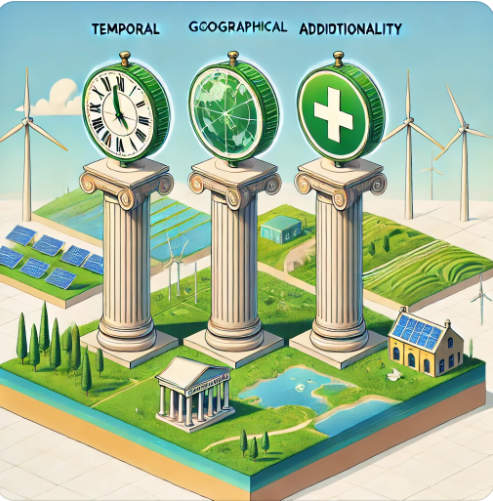
\includegraphics[width=1\linewidth]{images/3pillars}  
  		\source{ChatGPT4 hallucination, 2024}	
  \end{column}
  \end{columns}
 

  Iegor?
  
\end{frame}

\section{I Pillar - Temporal matching}
\begin{frame}{I Pillar: Temporal matching}
	\textbf{Discussion}: Implementing stricter regulations requires assessing the impact on hydrogen production costs.
	\begin{columns}[t]
		\begin{column}{0.5\textwidth}
			\centering
				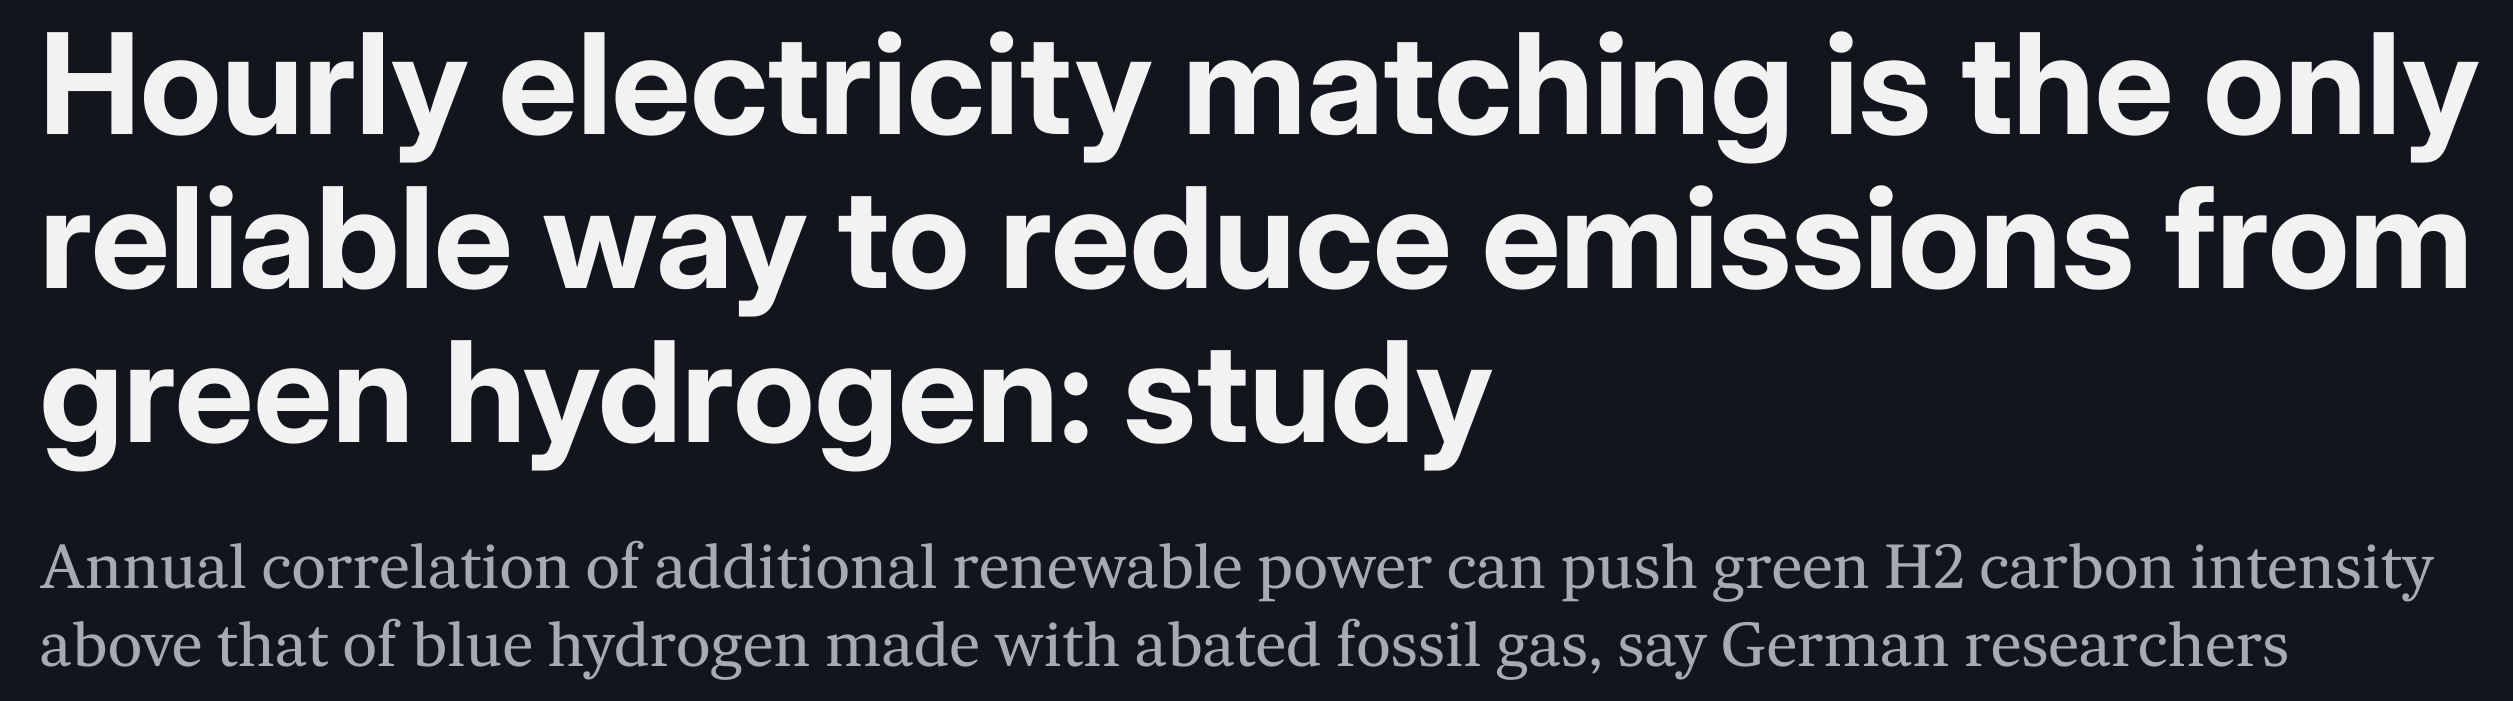
\includegraphics[width=5cm]{images/h2_temporal_news4}
				\newline
				\vspace{0.2cm}
				\newline
				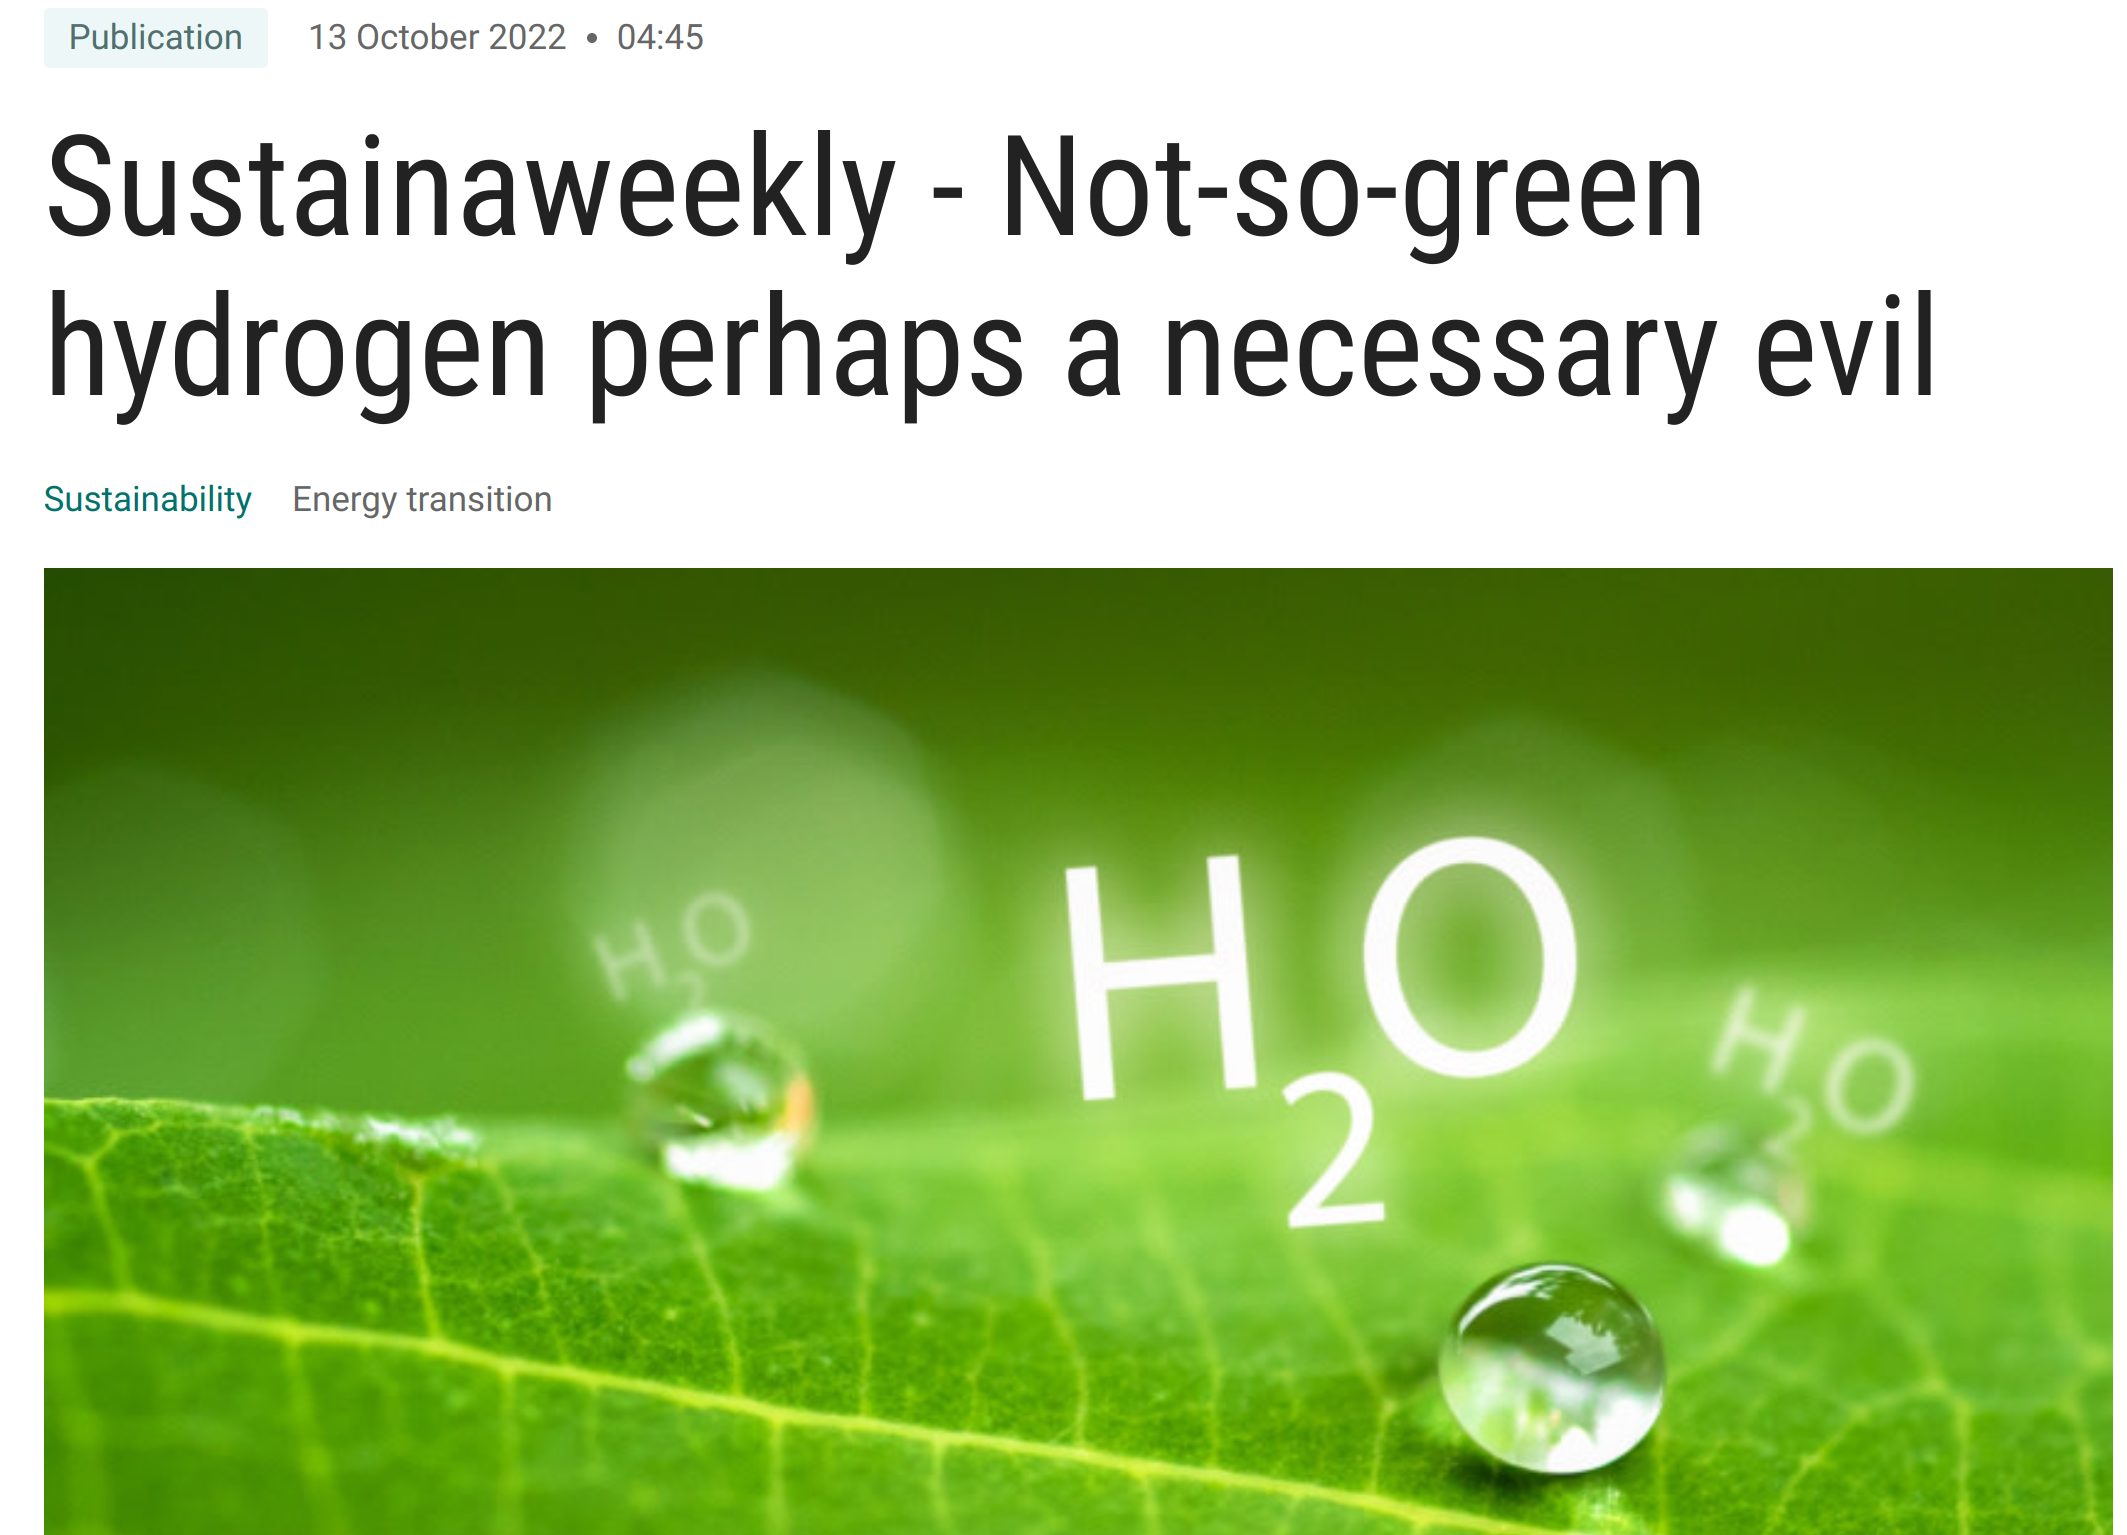
\includegraphics[width=4cm]{images/h2_temporal_news1}
		\end{column}
	\begin{column}{0.5\textwidth}
		\centering
		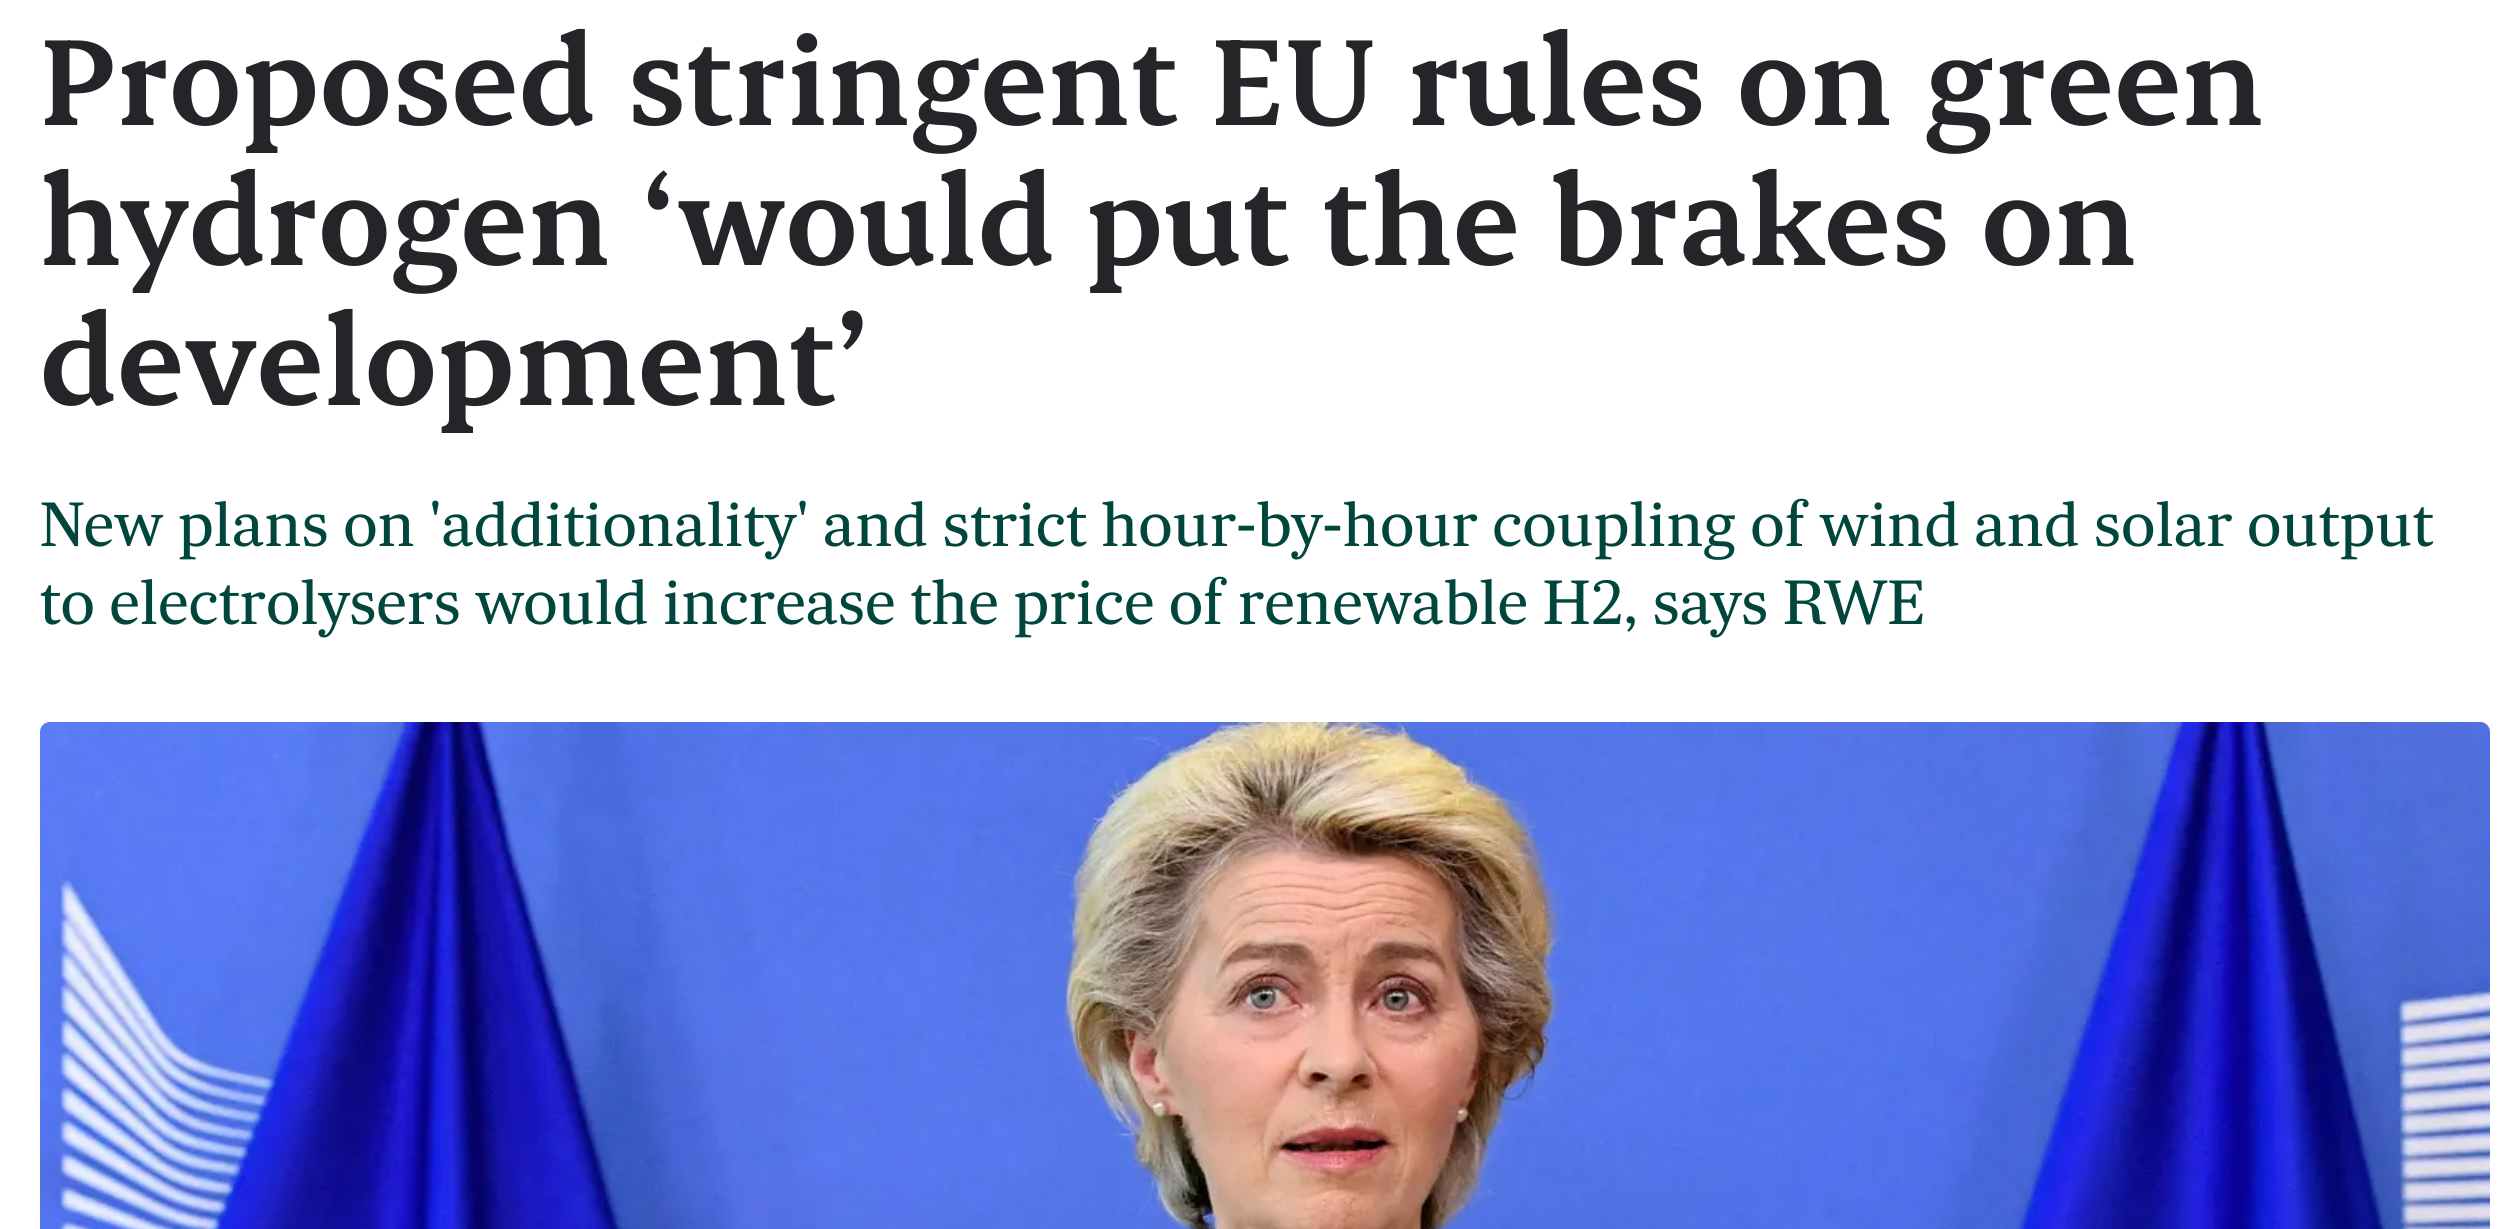
\includegraphics[width=5cm]{images/h2_temporal_news2}
		\newline
		\vspace{0.4cm}
		\centering
		\newline
		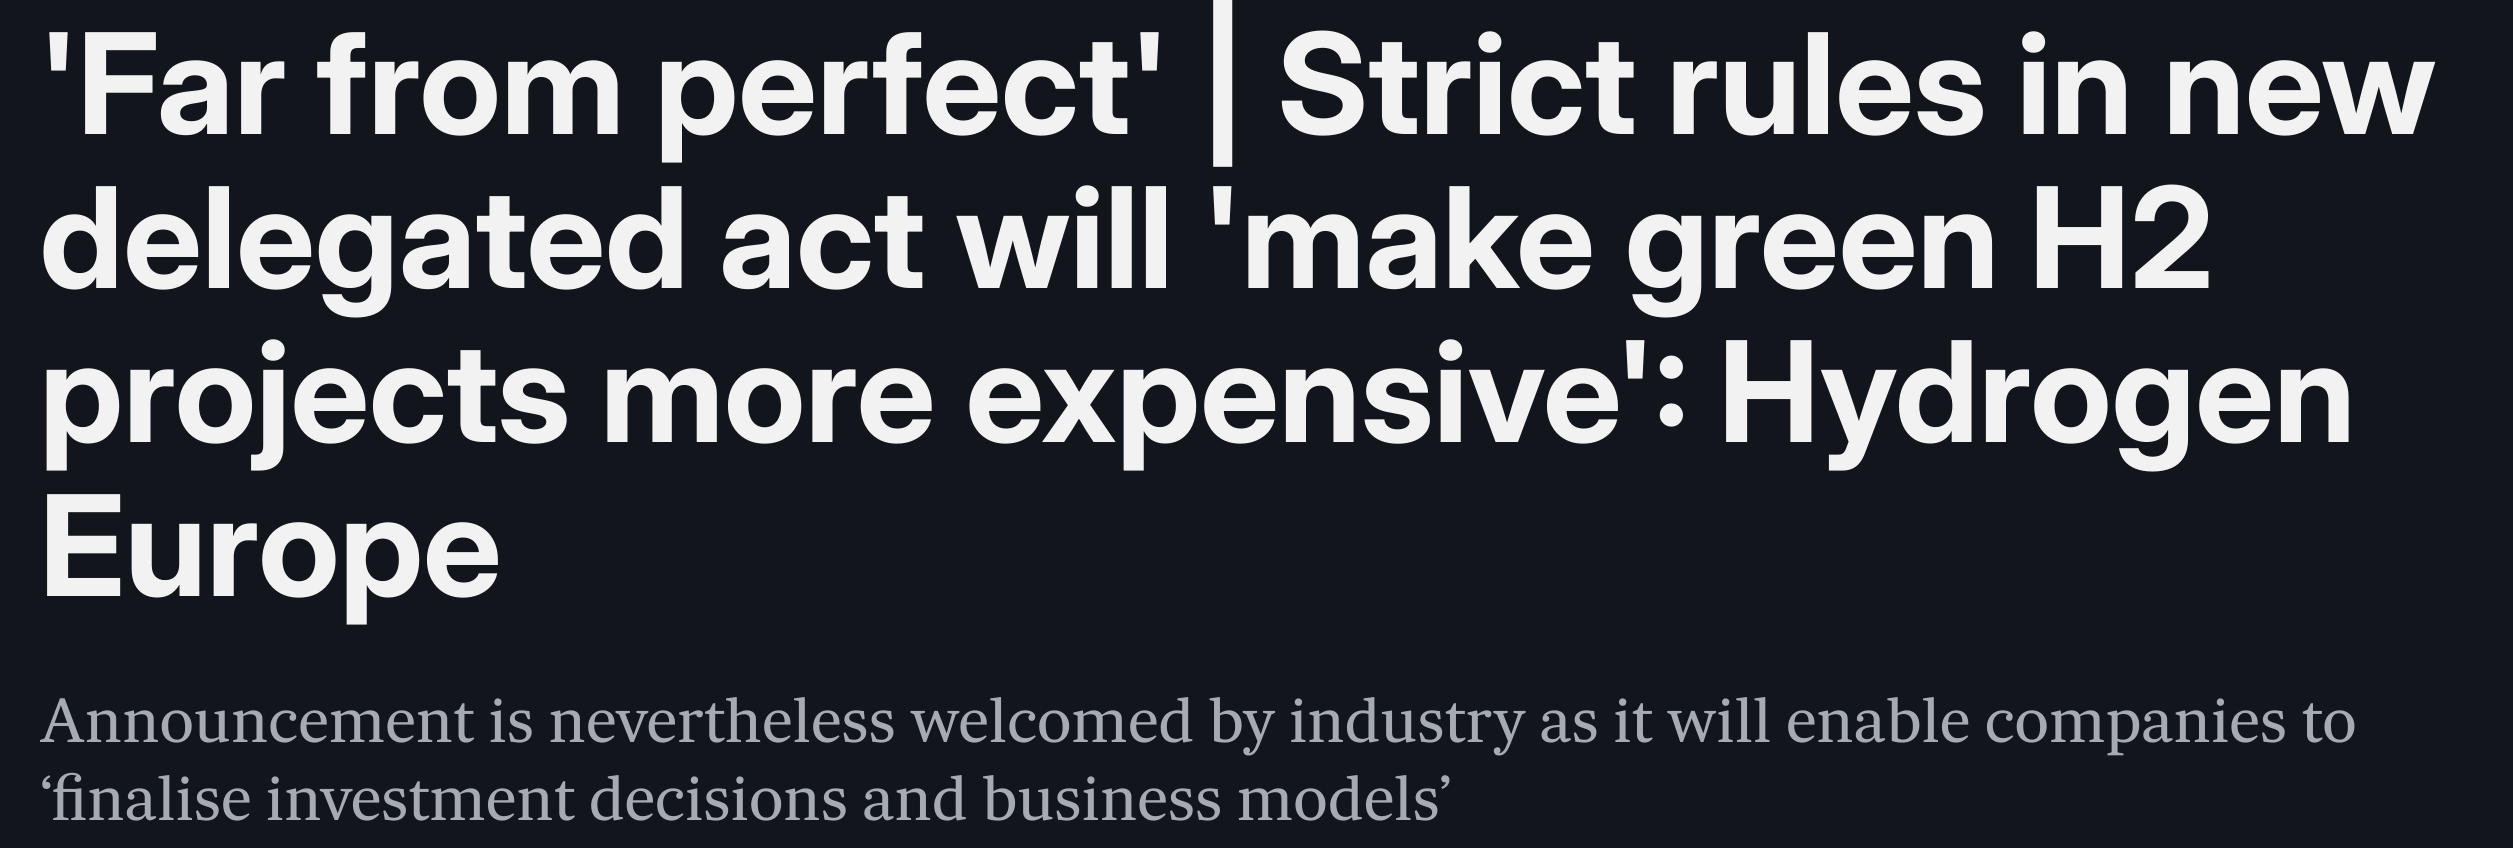
\includegraphics[width=5cm]{images/h2_temporal_news3}
		
	\end{column}
	\end{columns}
\source{\href{https://www.hydrogeninsight.com/policy/far-from-perfect-strict-rules-in-new-delegated-act-will-make-green-h2-projects-more-expensive-hydrogen-europe/2-1-1403241}{Hydrogeninsight (February 2023)}, \href{https://www.abnamro.com/research/en/our-research/sustainaweekly-not-so-green-hydrogen-perhaps-a-necessary-evil}{Abnamro (October 2022)}, \href{https://www.rechargenews.com/energy-transition/proposed-stringent-eu-rules-on-green-hydrogen-would-put-the-brakes-on-development-/2-1-1223746}{rechargenews (May 2022)}, \href{https://www.hydrogeninsight.com/policy/far-from-perfect-strict-rules-in-new-delegated-act-will-make-green-h2-projects-more-expensive-hydrogen-europe/2-1-1403241}{Hydrogeninsight (February 2023)}}
\end{frame}
\begin{frame}{Temporal matching: definition}
	
	\alert{Hourly matching} is modelled with a constraint, 
	which matches electricity demand for electrolysis process with generation of renewable resources on an hourly basis. 
	\centering
	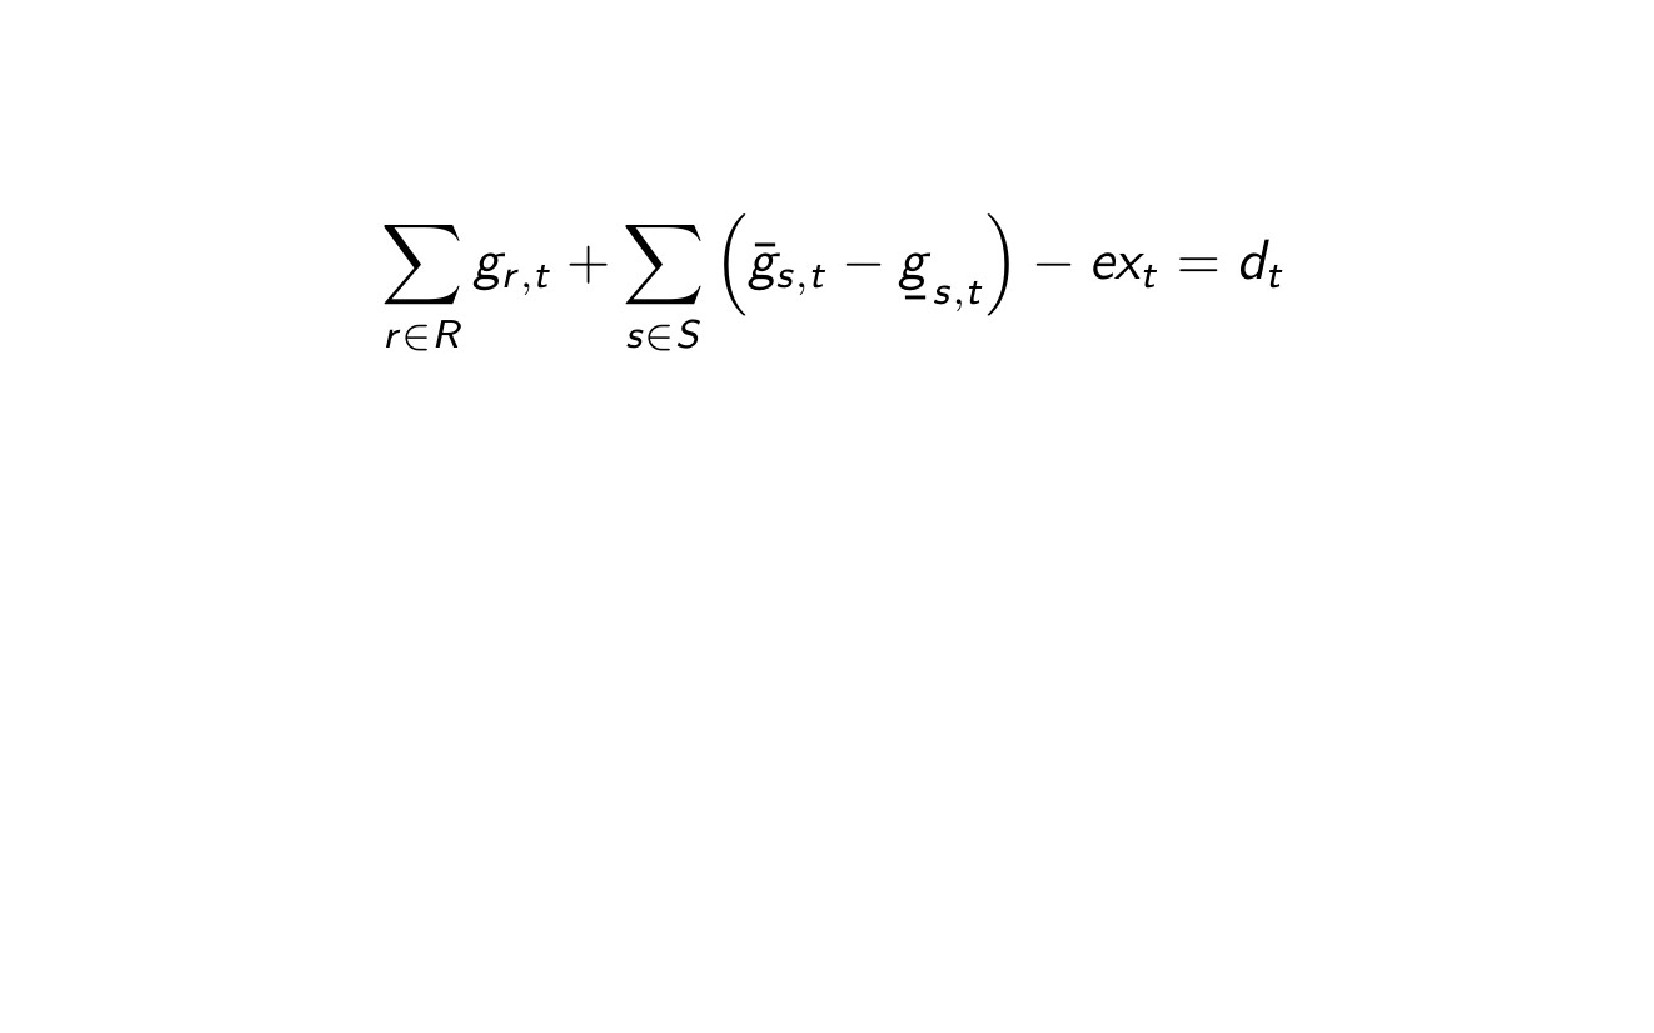
\includegraphics[width=0.6\linewidth, clip, trim={0cm 0cm 0cm 0cm}]{images/hourly_eq_explained_v0}

	\source{\href{https://iopscience.iop.org/article/10.1088/1748-9326/ad2239}{Zeyen et al. (2023): Temporal regulation \\ of renewable supply for electrolytic hydrogen}}

\end{frame}
\begin{frame}{Temporal matching: definition}
	\addtocounter{framenumber}{-1}
	\alert{Hourly matching} is modelled with a constraint, 
	which matches electricity demand for electrolysis process with generation of renewable resources on an hourly basis. 
	\centering
	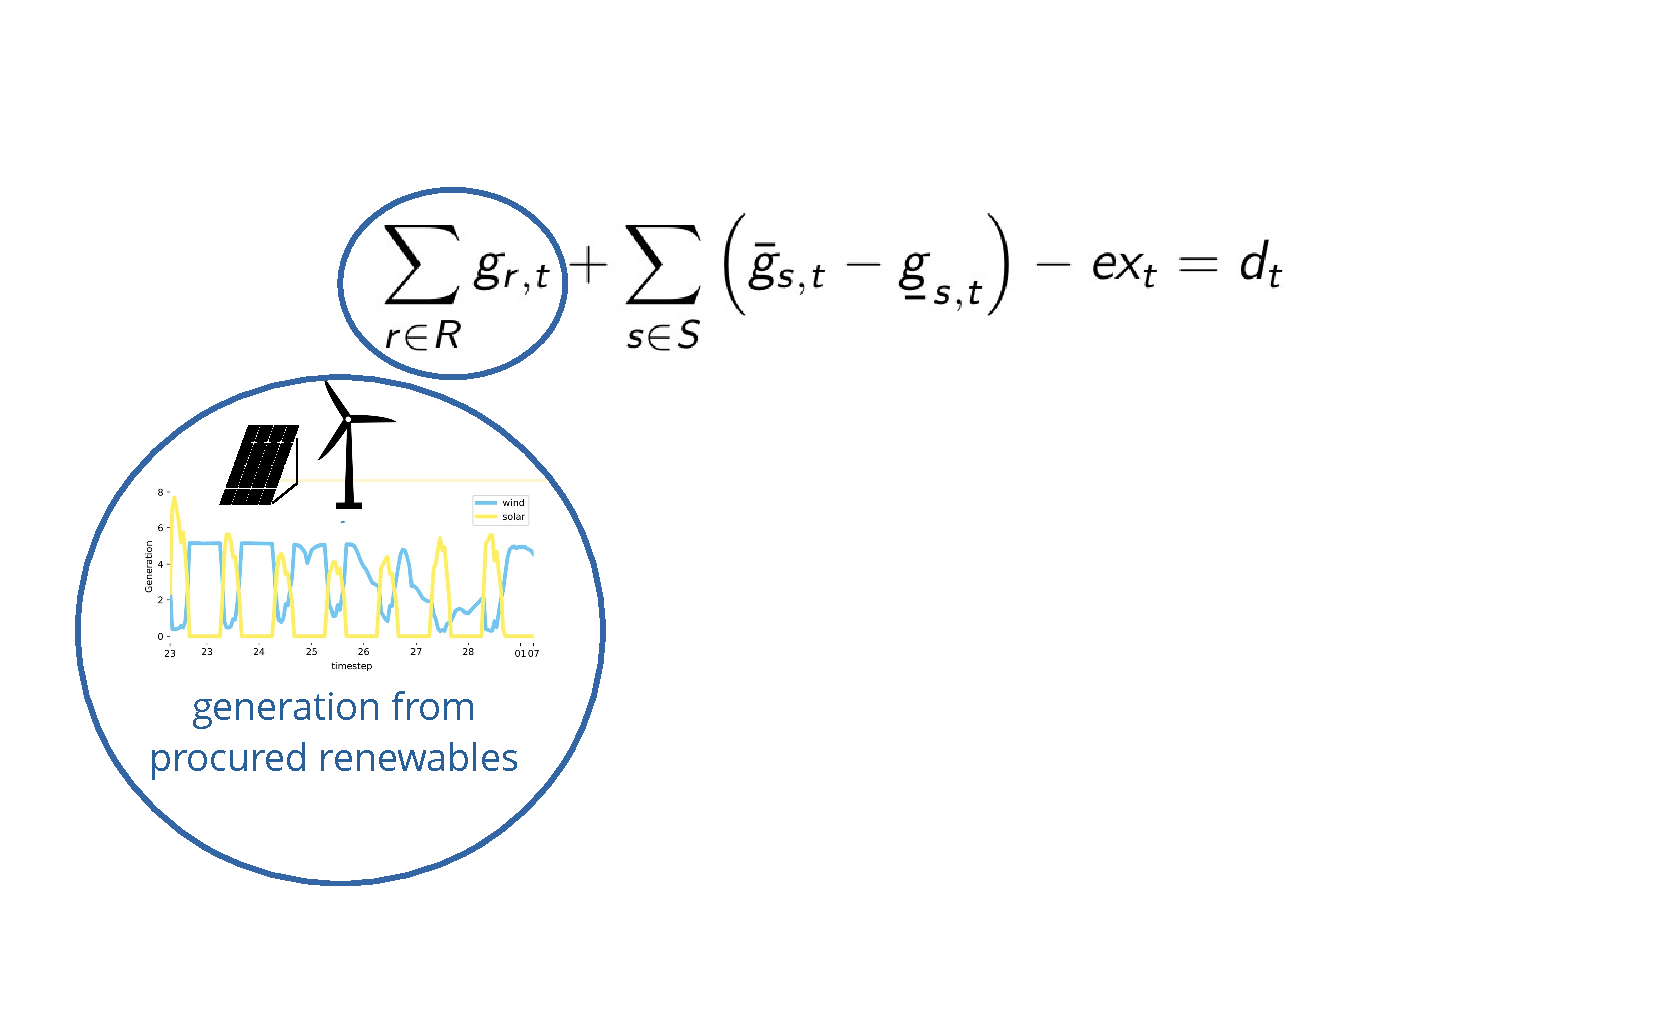
\includegraphics[width=0.6\linewidth, clip, trim={0cm 0cm 0cm 0cm}]{images/hourly_eq_explained_v1}
	
	\source{\href{https://iopscience.iop.org/article/10.1088/1748-9326/ad2239}{Zeyen et al. (2023): Temporal regulation \\ of renewable supply for electrolytic hydrogen}}

\end{frame}
\begin{frame}{Temporal matching: definition}
	\addtocounter{framenumber}{-1}
	\alert{Hourly matching} is modelled with a constraint, 
	which matches electricity demand for electrolysis process with generation of renewable resources on an hourly basis. 
	\centering
	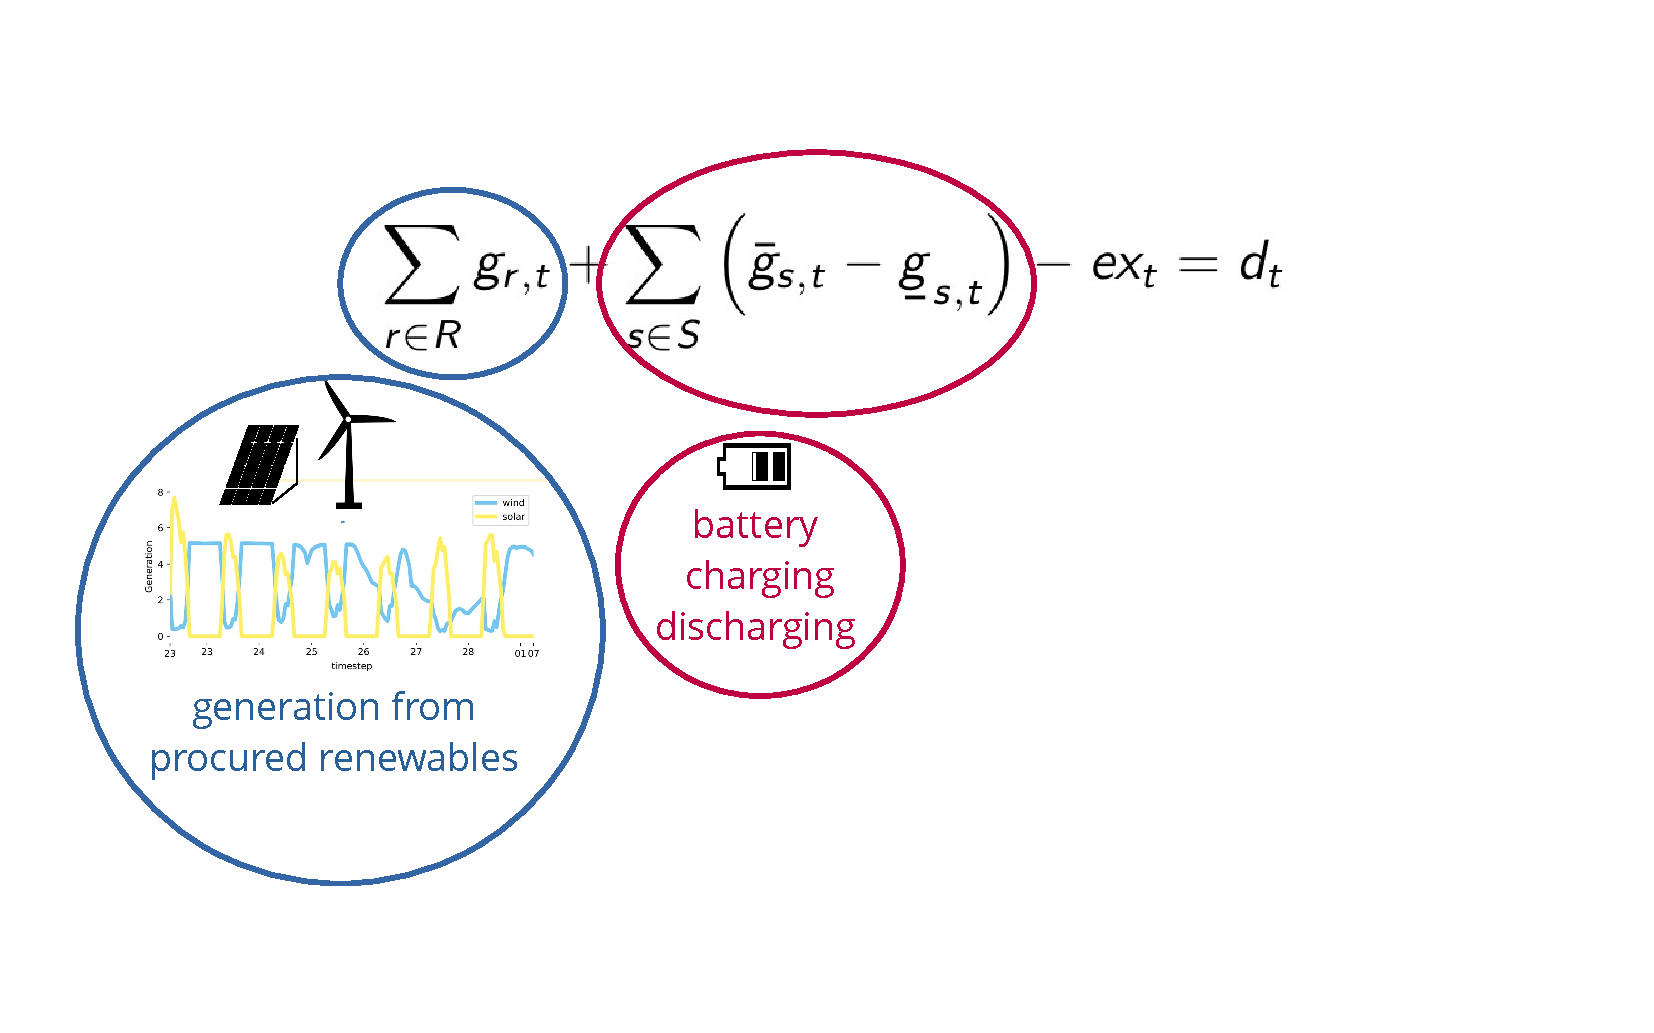
\includegraphics[width=0.6\linewidth, clip, trim={0cm 0cm 0cm 0cm}]{images/hourly_eq_explained_v2}
	
	\source{\href{https://iopscience.iop.org/article/10.1088/1748-9326/ad2239}{Zeyen et al. (2023): Temporal regulation \\ of renewable supply for electrolytic hydrogen}}

\end{frame}
\begin{frame}{Temporal matching: definition}
	\addtocounter{framenumber}{-1}
	\alert{Hourly matching} is modelled with a constraint, 
	which matches electricity demand for electrolysis process with generation of renewable resources on an hourly basis. 
	\centering
	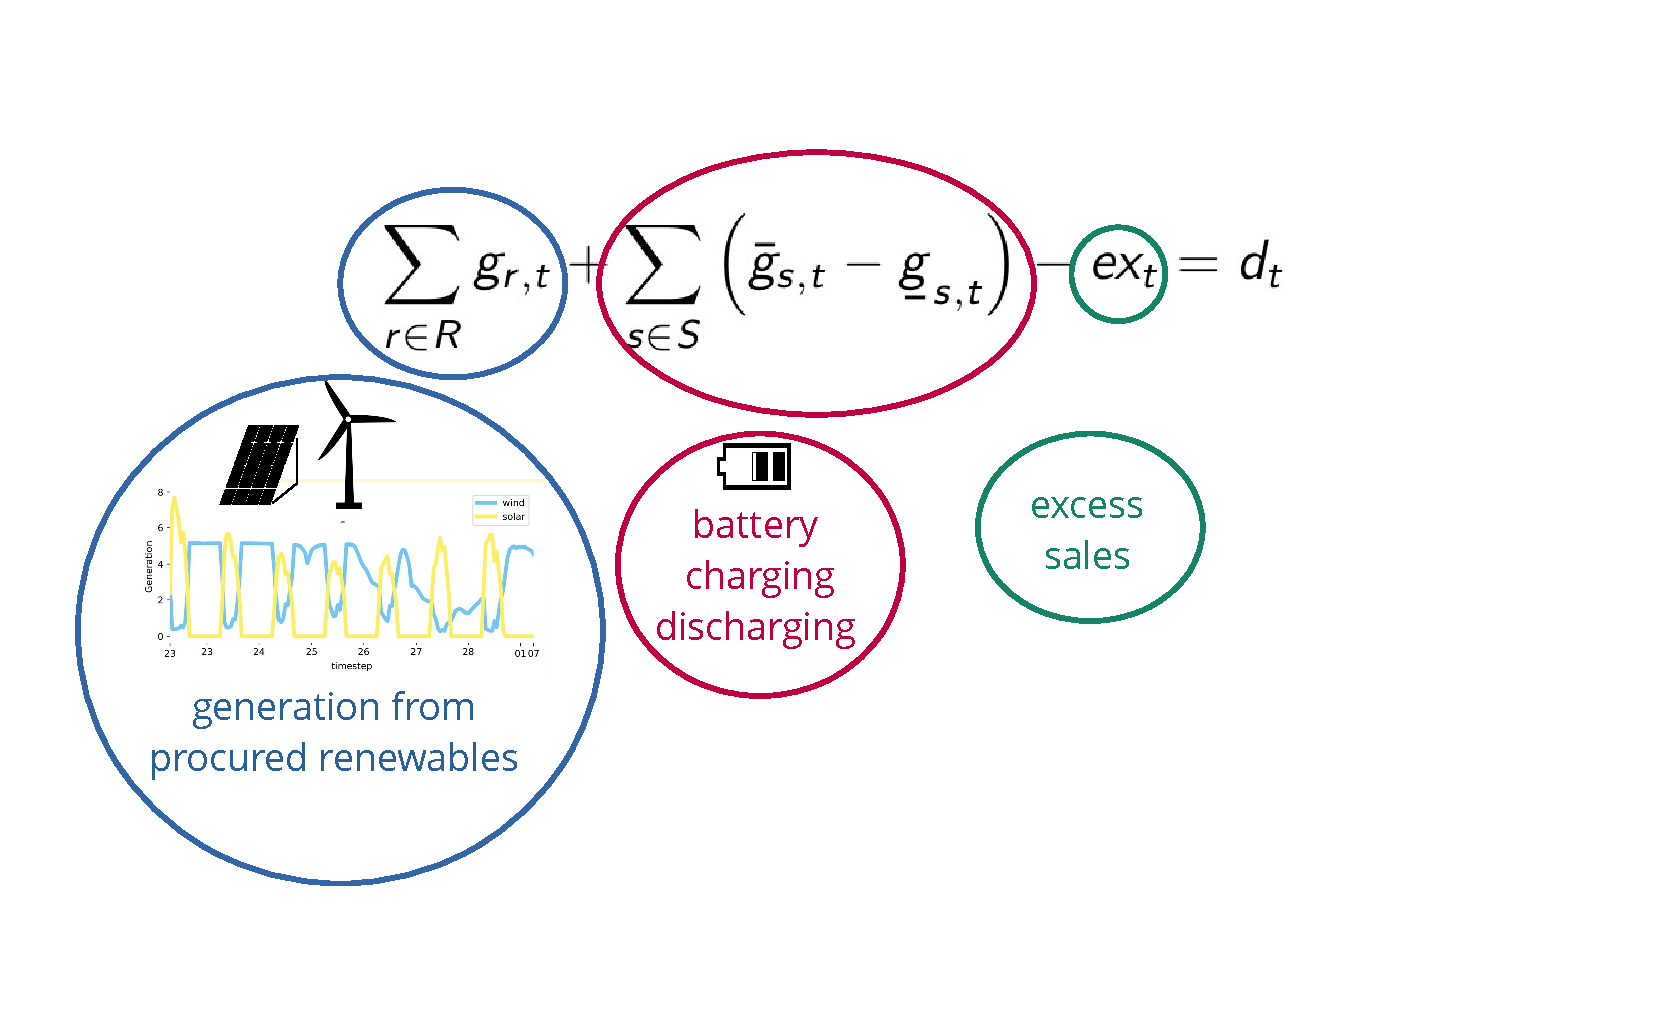
\includegraphics[width=0.6\linewidth, clip, trim={0cm 0cm 0cm 0cm}]{images/hourly_eq_explained_v3}
	
	\source{\href{https://iopscience.iop.org/article/10.1088/1748-9326/ad2239}{Zeyen et al. (2023): Temporal regulation \\ of renewable supply for electrolytic hydrogen}}

\end{frame}
\begin{frame}{Temporal matching: definition}
\addtocounter{framenumber}{-1}
  \alert{Hourly matching} is modelled with a constraint, 
  which matches electricity demand for electrolysis process with generation of renewable resources on an hourly basis. 

%  \vspace{0.1cm}
%  \begin{equation}
%  \sum_{r\in R} g_{r,t} + \sum_{s\in S} \left(\bar{g}_{s,t} - \ubar{g}_{s,t}\right) - ex_t = d_t
%  \label{eqn:CFE_1}
%  \end{equation}
%  \vspace{0.1cm}
  \centering
  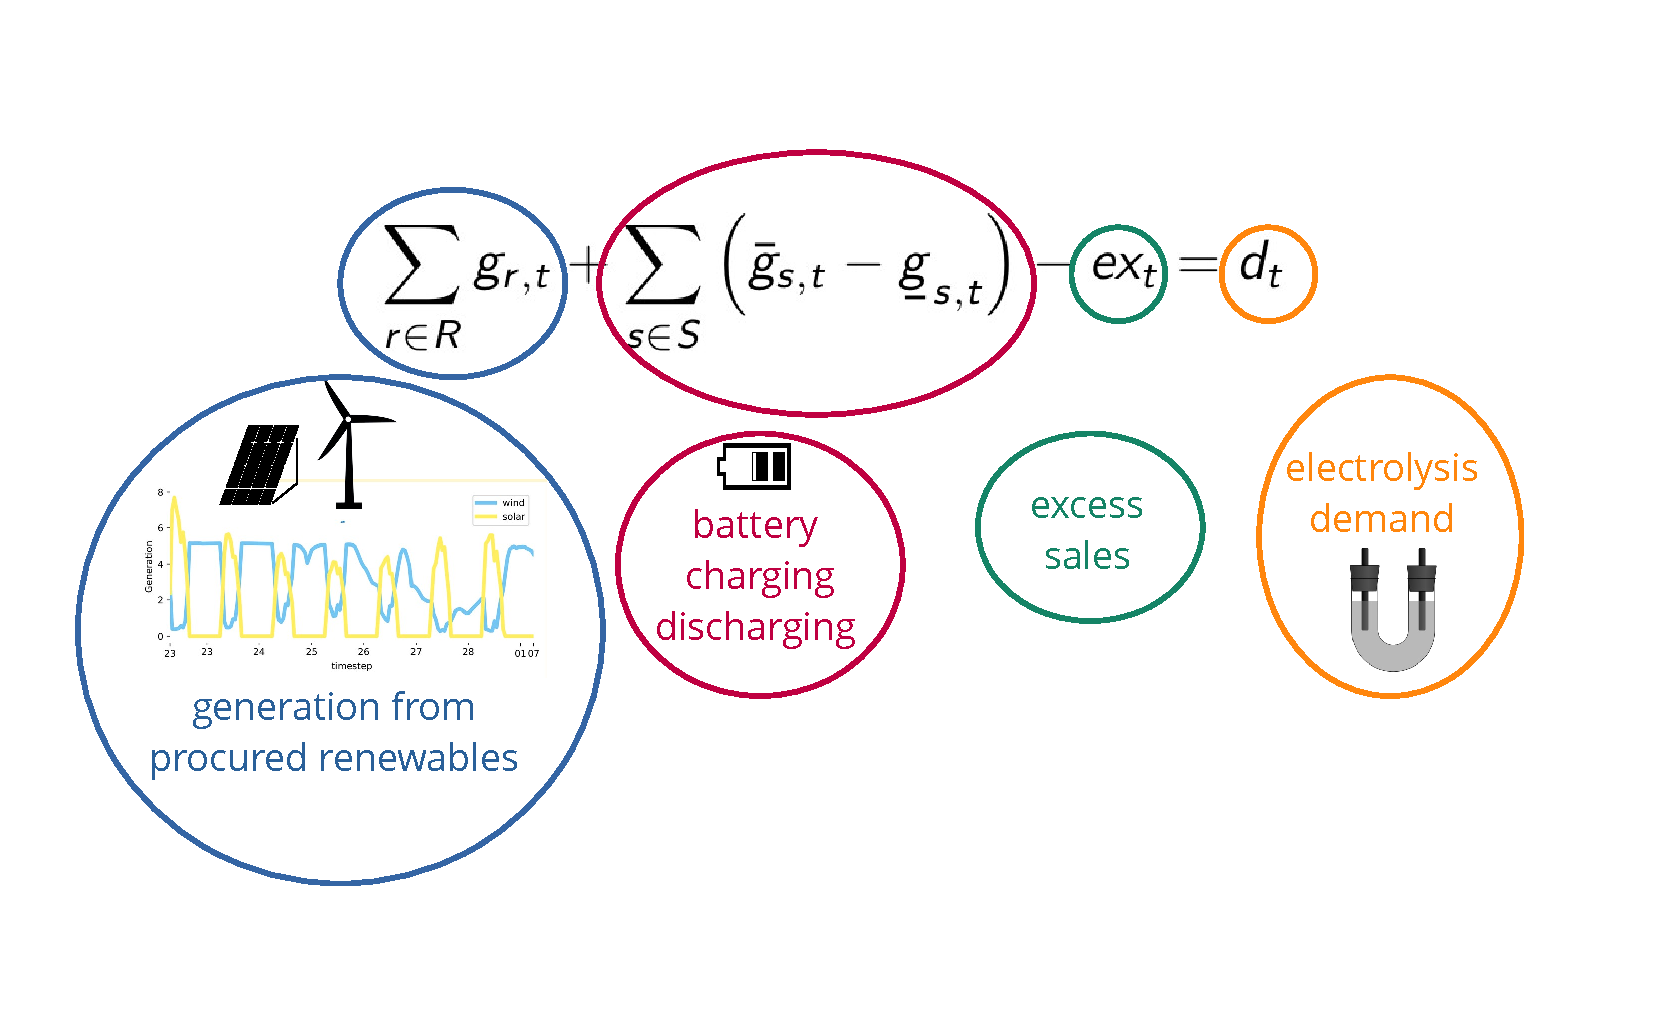
\includegraphics[width=0.6\linewidth, clip, trim={0cm 0cm 0cm 0cm}]{images/hourly_eq_explained}
%  \noindent\fbox{%
%    \parbox{\textwidth}{%
%  Here eq. 2 from https://iopscience.iop.org/article/10.1088/1748-9326/ad2239/pdf \\
%  -- maybe here we say along the lines that the main fight in the Delegated Act was for this equation. \\
%  -- explain the equation\\ 
%  -- Now, what are the hidden issues? let's talk about the first point -- flexibility. \\
%  }}
  \source{\href{https://iopscience.iop.org/article/10.1088/1748-9326/ad2239}{Zeyen et al. (2023): Temporal regulation \\ of renewable supply for electrolytic hydrogen}}
\end{frame}


\begin{frame}{Temporal matching: flexibility changes everything}
	\vspace{-5cm} 
	\centering
	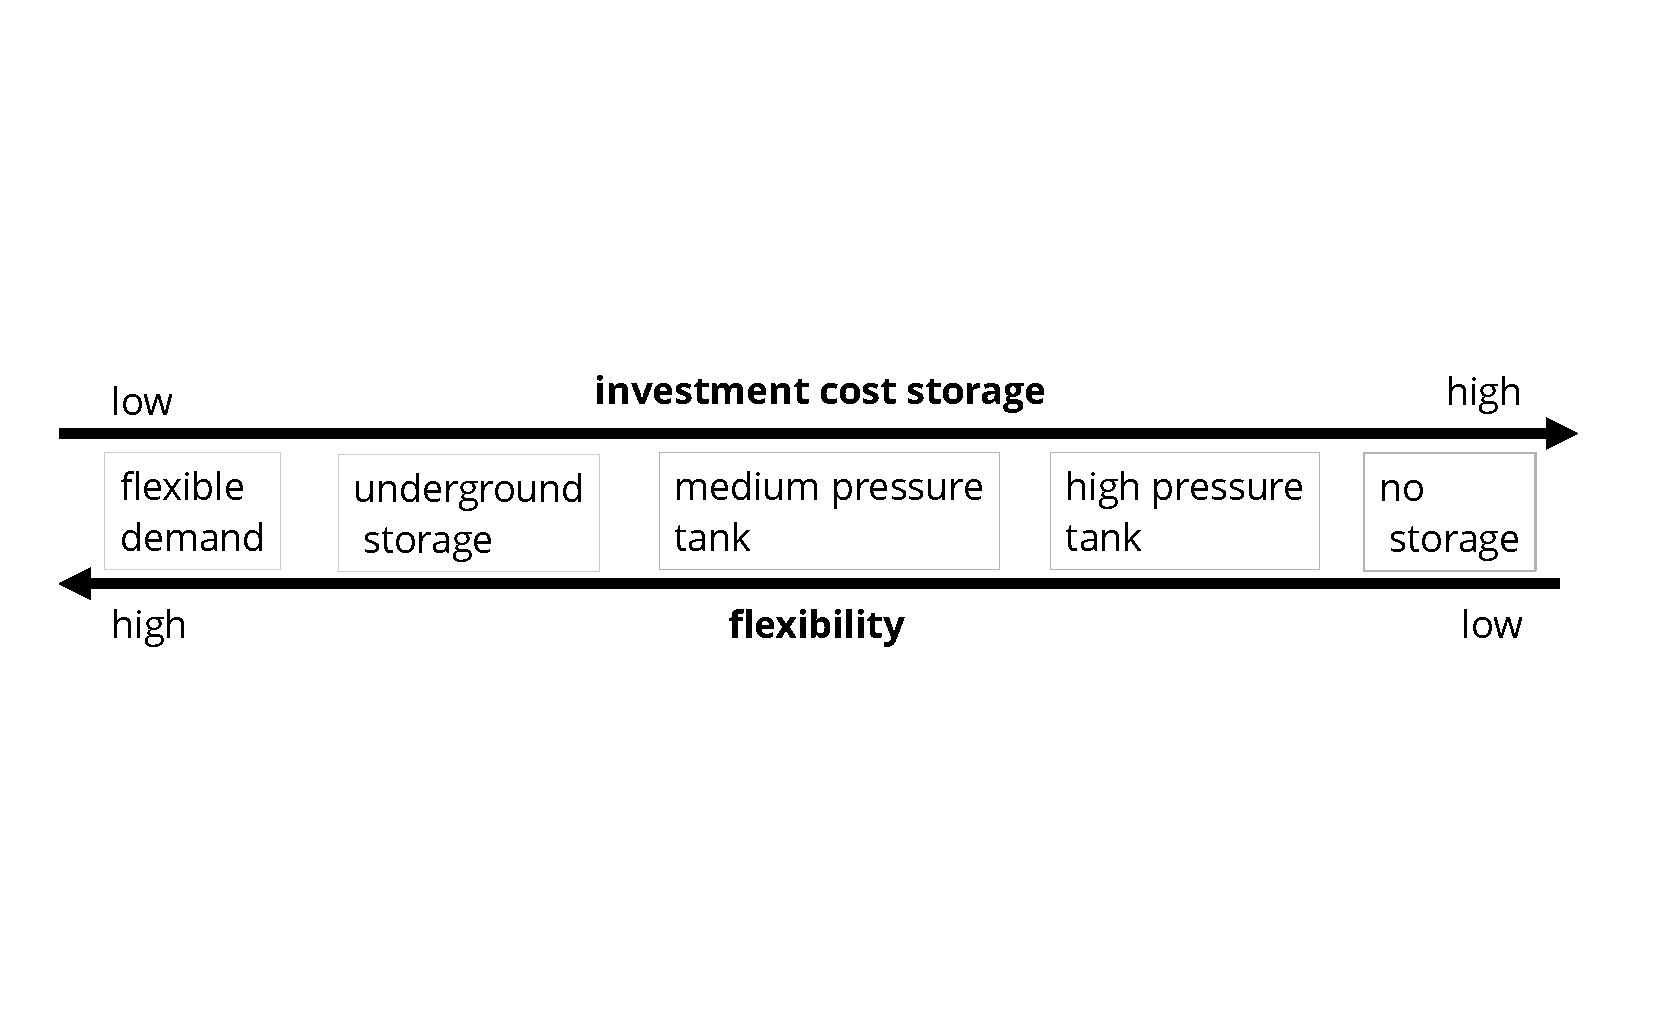
\includegraphics[width=0.6\linewidth, clip, trim={0cm 5cm 0cm 5cm}]{images/store_flexibility_v2}


	\source{\href{https://iopscience.iop.org/article/10.1088/1748-9326/ad2239}{Zeyen et al. (2023): Temporal regulation \\ of renewable supply for electrolytic hydrogen}}
\end{frame}

\begin{frame}{Temporal matching: flexibility changes everything}
	\addtocounter{framenumber}{-1}
	\vspace{-1cm} 
	\centering
	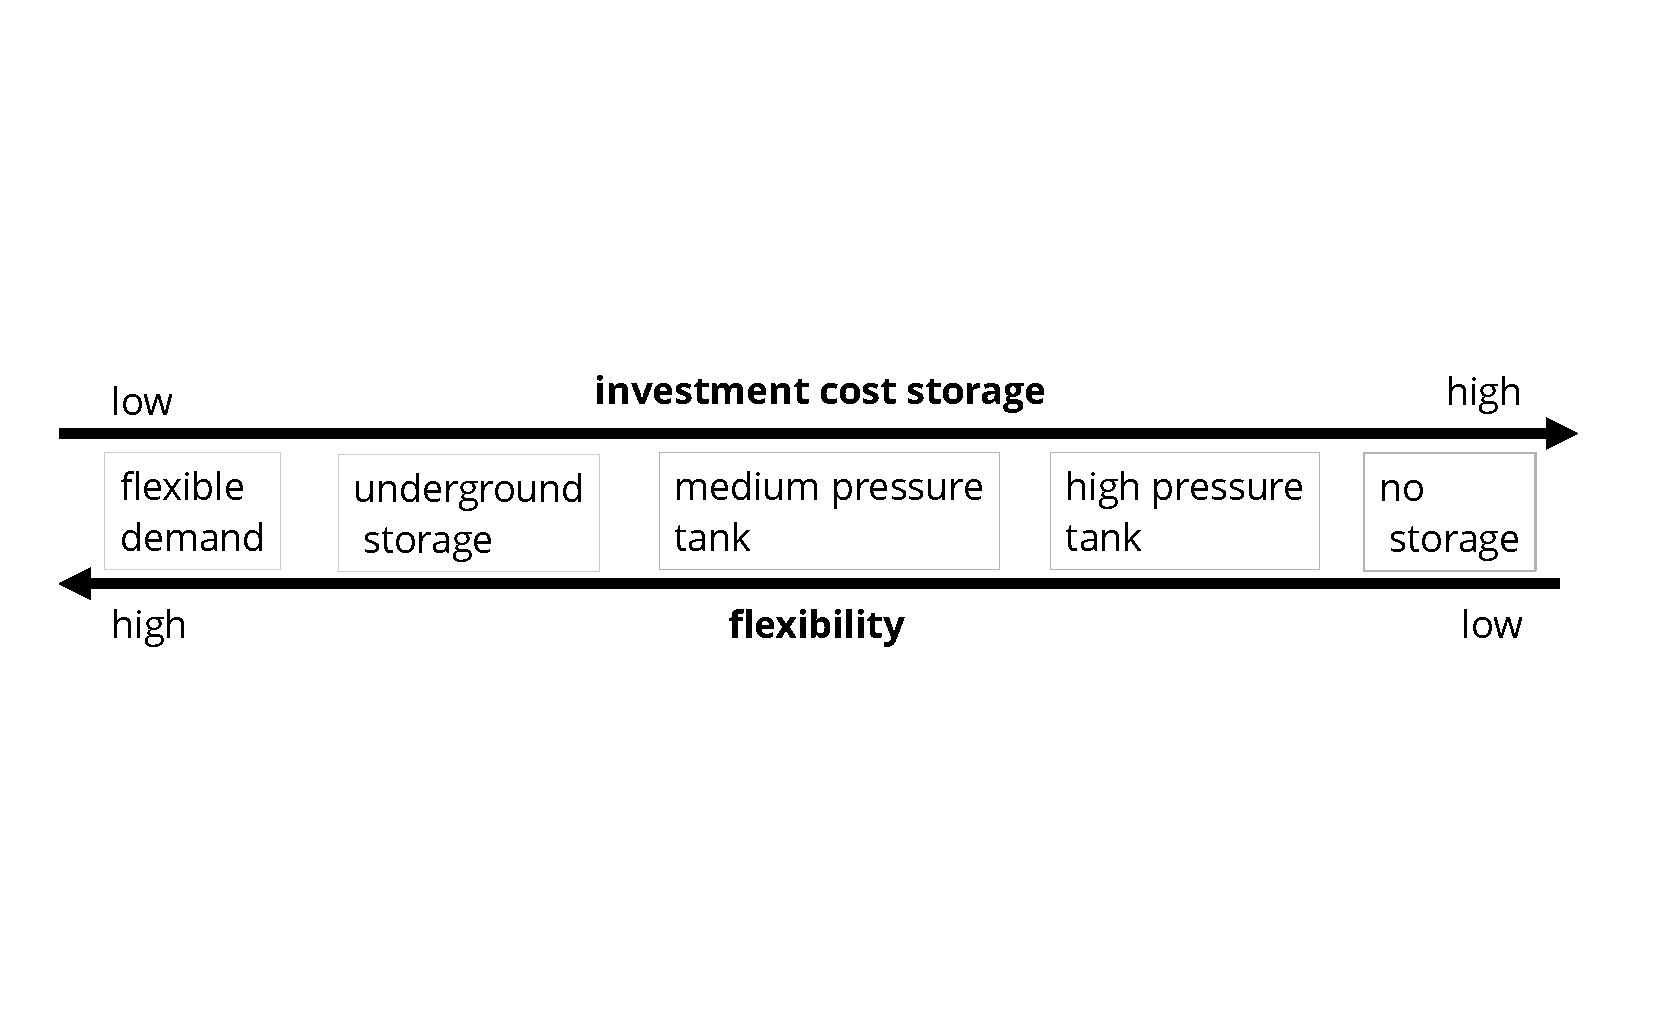
\includegraphics[width=0.6\linewidth, clip, trim={0cm 5cm 0cm 5cm}]{images/store_flexibility_v2}
	\begin{columns}[t]
		\begin{column}{0.5\textwidth}
			\centering
				\textbf{Emissions} \\
				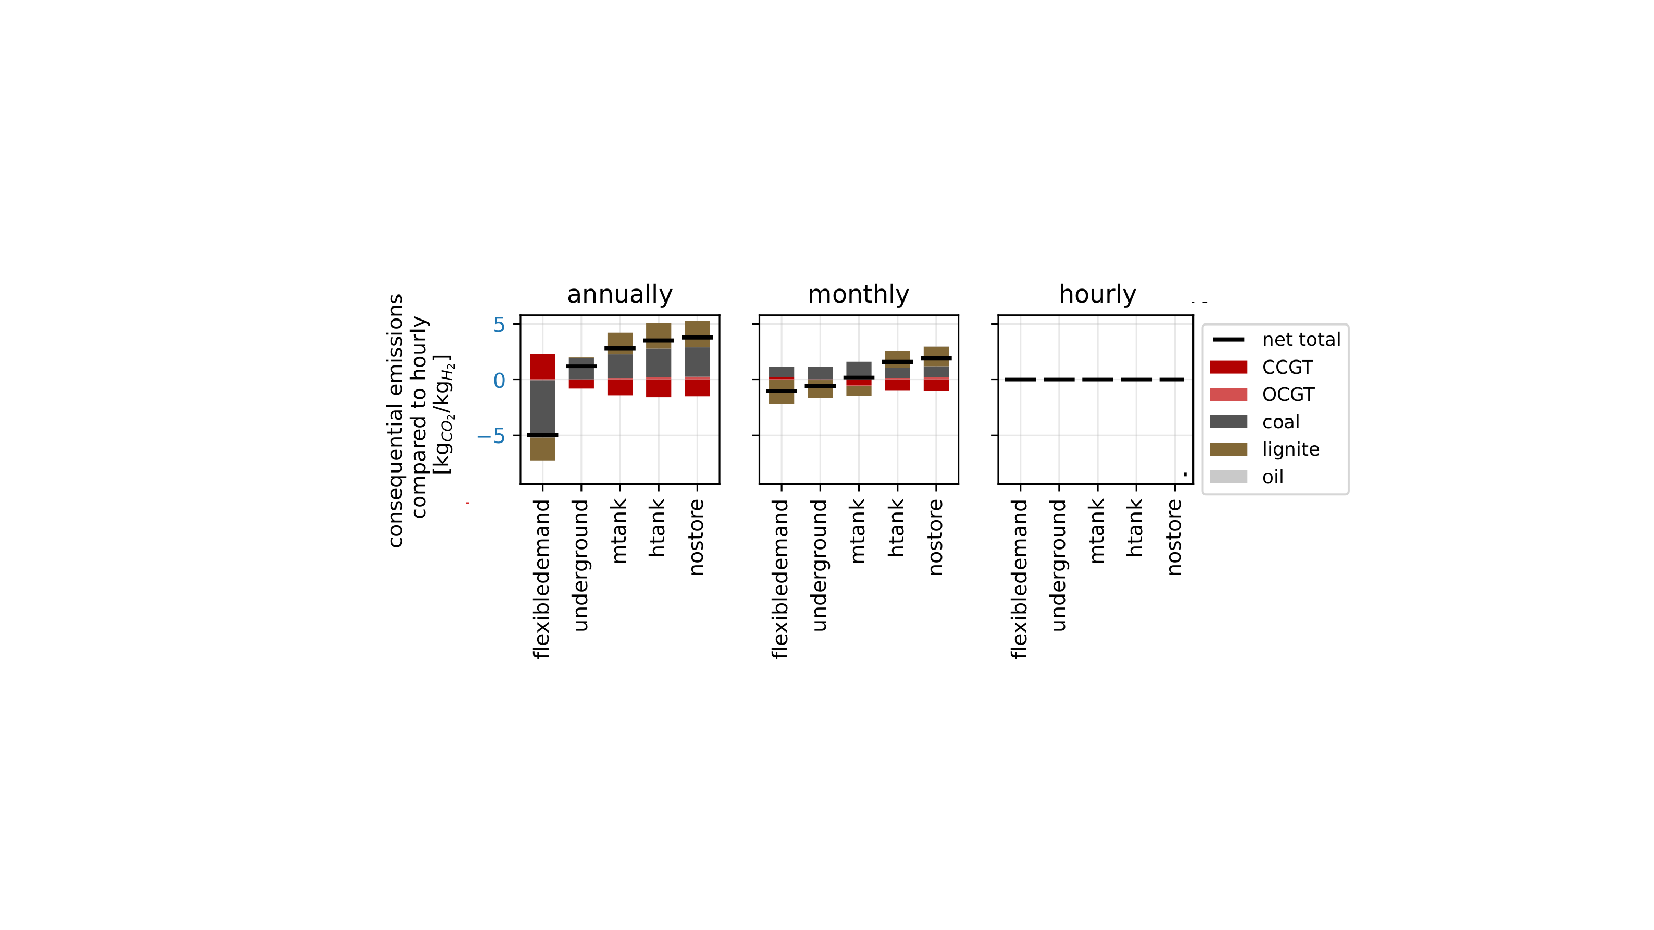
\includegraphics[width=1\linewidth, clip, trim={5cm 4cm 5cm 4cm}]{images/emissions_flexibility}
		\end{column}
		\begin{column}{0.5\textwidth}
				\textbf{Hydrogen production costs} \\
				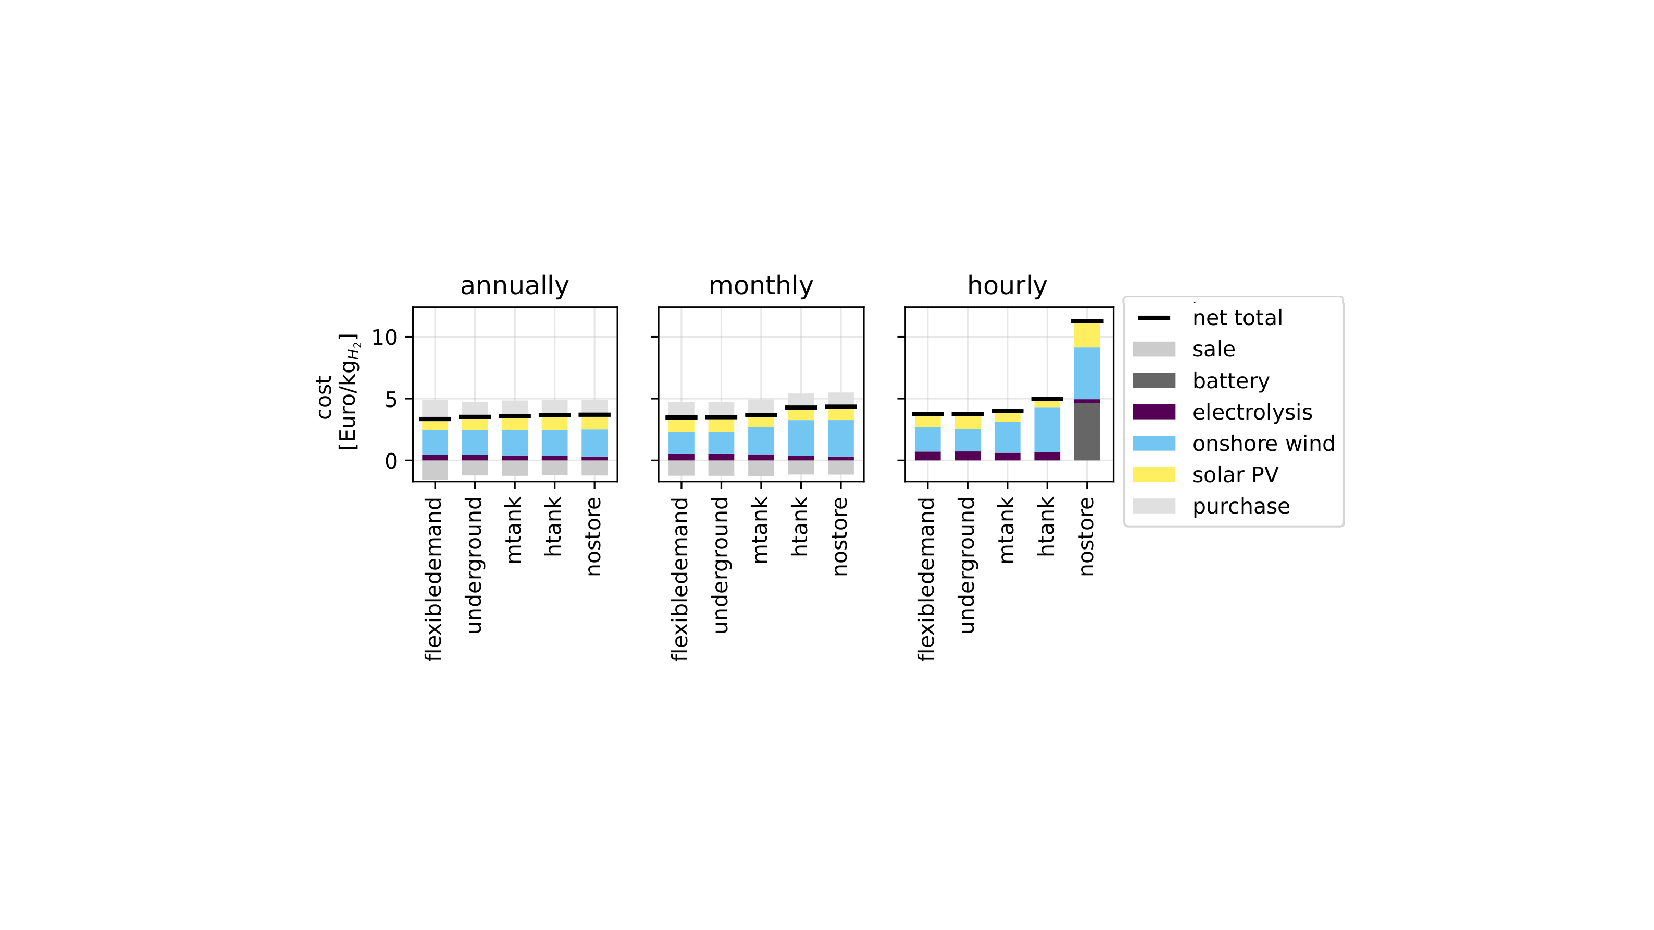
\includegraphics[width=1\linewidth, clip, trim={5cm 4cm 5cm 4cm}]{images/costs_flexibility}
		\end{column}
	\end{columns}

	Flexibility \alert{reduces} emissions and costs.
	\source{\href{https://iopscience.iop.org/article/10.1088/1748-9326/ad2239}{Zeyen et al. (2023): Temporal regulation \\ of renewable supply for electrolytic hydrogen}}
\end{frame}

\begin{frame}{Temporal matching: higher excess sales reduce emissions and costs}
	\centering
	\vspace{-2cm}
	The \alert{costs of hydrogen production decrease} by up to 30\% in case of flexible demand + hourly matching due to the larger profits from excess sales.
	\vspace{0.5cm}
  	\begin{columns}[t]
  	\begin{column}{0.5\textwidth}
  		\centering
  		\textbf{Annual} \\
  		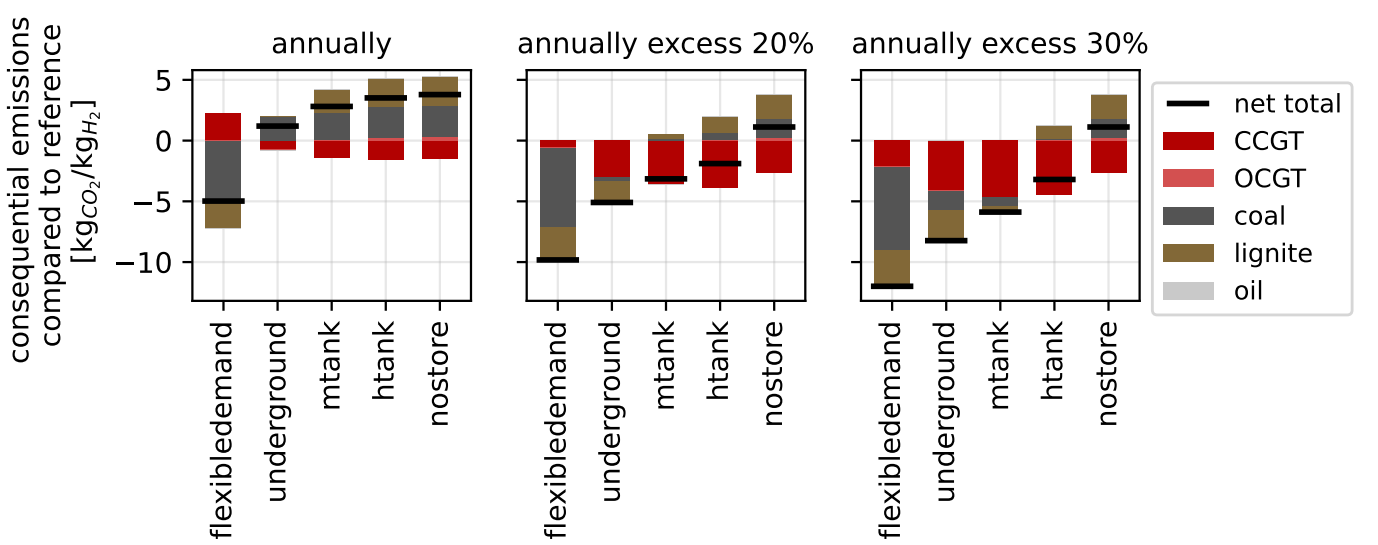
\includegraphics[width=1\linewidth]{images/annual_excess}
  	\end{column}
  	\begin{column}{0.5\textwidth}
  		\centering
  		\textbf{Hourly} \\
  		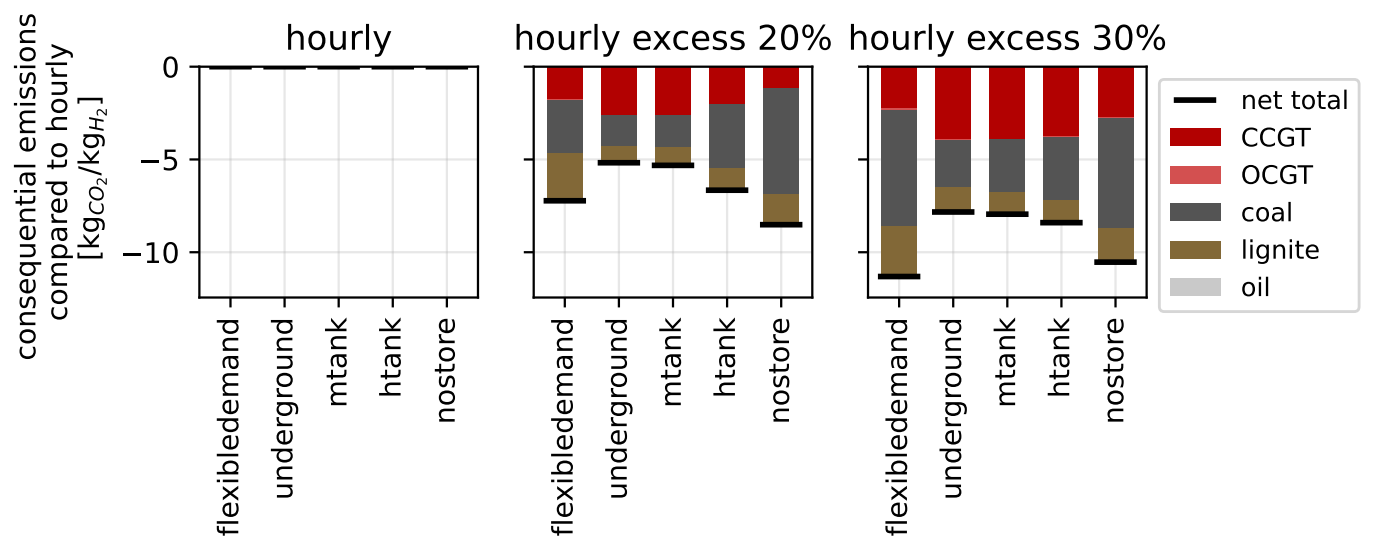
\includegraphics[width=1\linewidth]{images/hourly_excess}
  	\end{column}
  \end{columns}
  \source{\href{https://iopscience.iop.org/article/10.1088/1748-9326/ad2239}{Zeyen et al. (2023): Temporal regulation \\ of renewable supply for electrolytic hydrogen}}

\end{frame}


\begin{frame}{Temporal matching: (CFE story)}

  Here, the \alert{hourly matching} constraint is extended to include electricity consumption from the regional grid:

  \vspace{0.1cm}
  \begin{equation}
  \sum_{r\in CFE, t\in T} g_{r,t} + \sum_{s\in STO, t\in T} \left(\bar{g}_{s,t} - \ubar{g}_{s,t}\right) - \sum_{t\in T} ex_t + \textcolor{red}{\sum_{t\in T} CFE_t \cdot im_t} \geq x \cdot \sum_{t\in T} d_t
  \label{eqn:CFE}
  \end{equation}
  \vspace{0.1cm}
  \source{Riepin \& Brown (2023): https://zenodo.org/records/7180098}

  \noindent\fbox{%
    \parbox{\textwidth}{%
    The \alert{grid CFE factor} $CFE_t$ in eq. (\ref{eqn:CFE}) defines the share of 
    carbon-free electricity in grid imports. \\
    -- depends how you scope out CFE calculation \\
    -- storage tracing \\
    -- CFE isn't a parameter but a variable \\
  }}
  Iegor

\end{frame}


\section{II Pillar - Geographical matching}
\begin{frame}{II Pillar - Geographical matching}
  Iegor?
  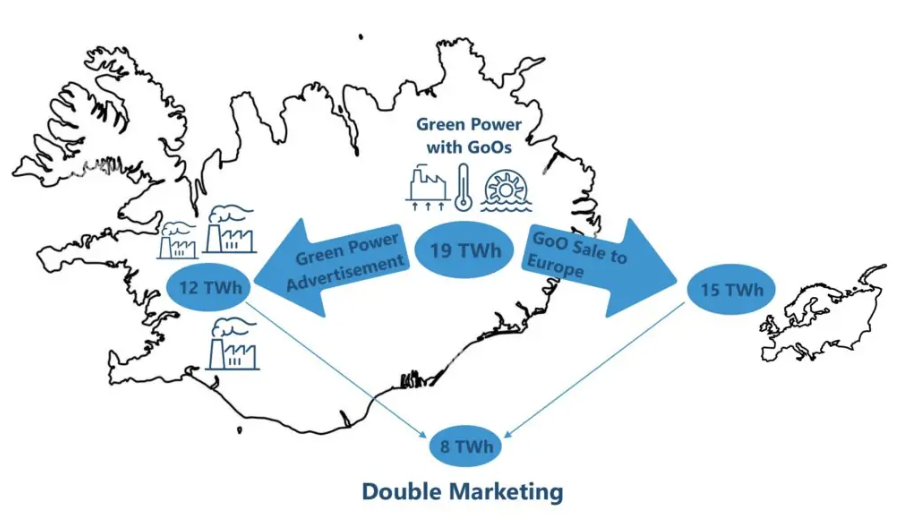
\includegraphics[width=13cm]{images/go_leak.png}
  \source{https://www.ffe.de/en/publications/norway-and-the-double-marketing-of-renewable-energies/}
\end{frame}



\begin{frame}{Geographical matching}

  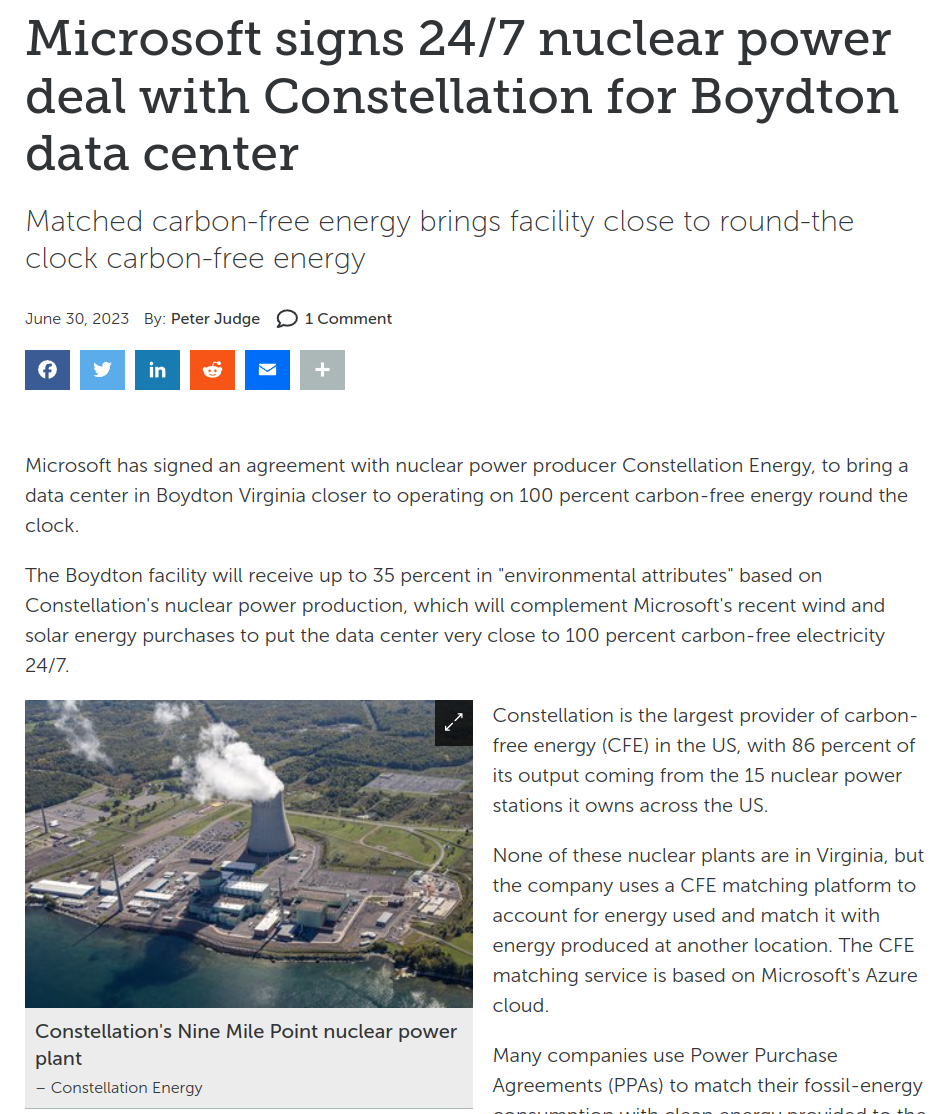
\includegraphics[width=8cm]{images/microsoft.png}
  \source{datacenterdynamics "Microsoft signs 24/7 nuclear power deal with Constellation for Boydton data center" (June 30, 2023)}

\end{frame}

\begin{frame}{Geographical matching}

  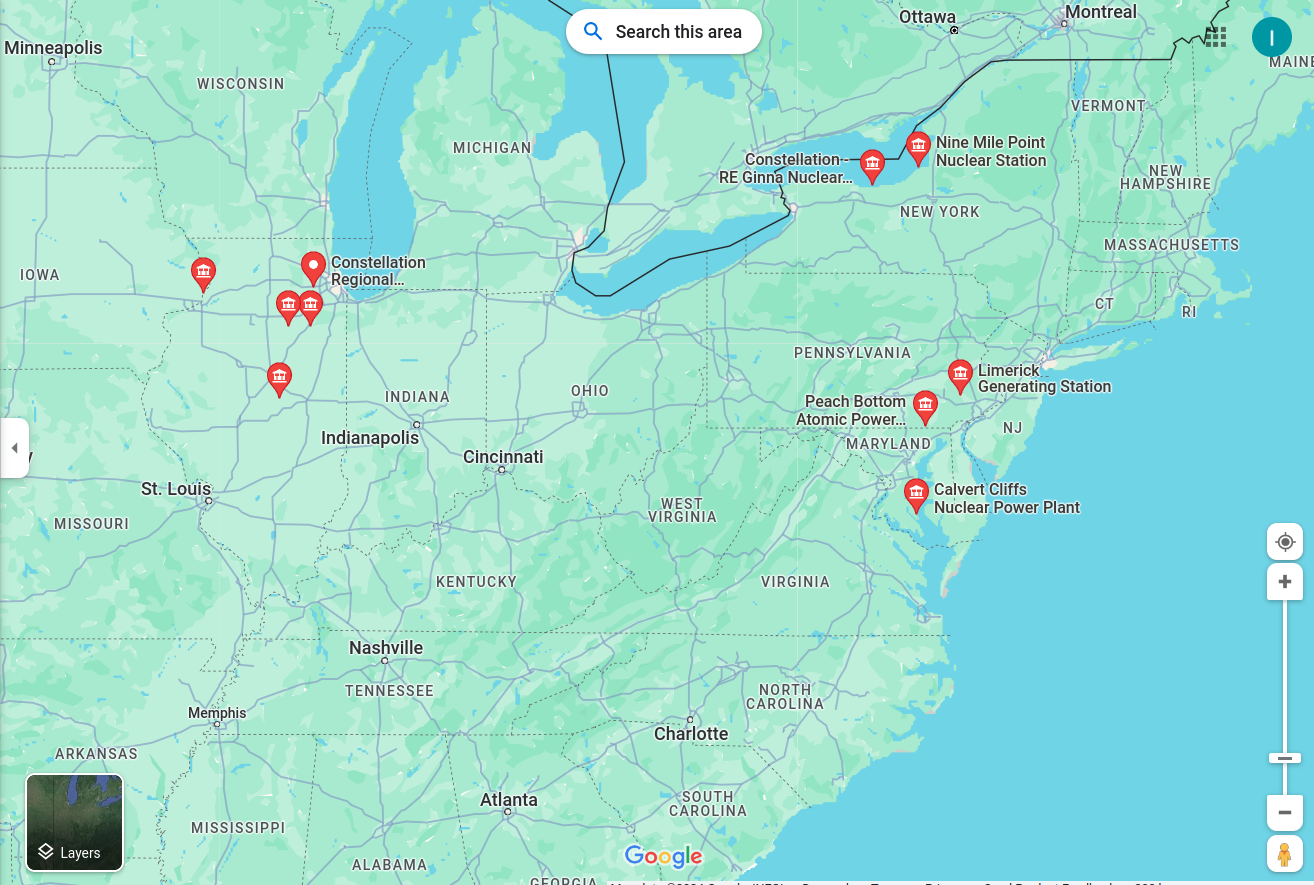
\includegraphics[width=13cm]{images/microsoft2.png}

\end{frame}
  

\begin{frame}{Geographical matching for green hydrogen production}
\begin{columns}
	\begin{column}{0.4\textwidth}
		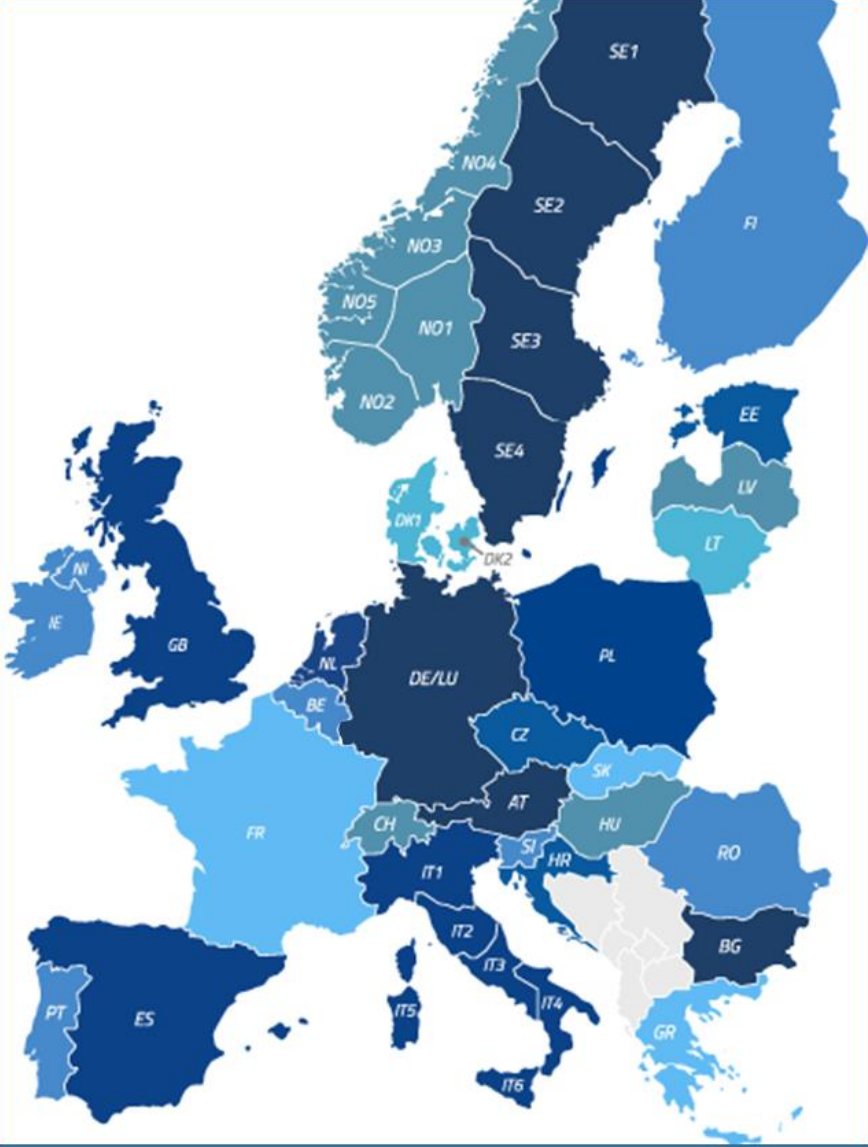
\includegraphics[width=5cm, clip, trim={0 0.1cm 0 0}]{images/biding_zones_eu.png}
		\source{\href{https://acer.europa.eu/sites/default/files/documents/en/Documents/Presentations\%20Webinars/20210624_Public_webinar_alternative_BZ_configurations.pdf}{ACER, 2021}}
	\end{column}
	\begin{column}{0.6\textwidth}
		How far can renewable generation and electrolysis be apart? 
		\begin{itemize}
			\item 	Regulation in the EU: Geographical matching within one \alert{bidding zone}.
			\item 	Model implementation is straightforward. 
		\end{itemize}

	\vspace{0.5 cm}
		\textbf{Challenges}: Especially in large bidding zones there can be \alert{transmission bottlenecks} actually hindering the transport of renewable generation to the electrolysis. 
	\end{column}
\end{columns}
\end{frame}

\section{III Pillar - Additionality}
\begin{frame}{III Pillar - Additionality}

  Iegor starts? 

  -- start with the fact that it's complex and messy both in real world and in models\\
  -- define it (over MW and MWh)\\
  -- as a funny reference, we can re-use the Microsoft PPA deal example with existing nuclear power.

\end{frame}


\begin{frame}{Additionality: definition challenges}

  Iegor or Elisabeth?\\
Different definitions:
\begin{itemize}
	\item \textbf{Google}:
	\item \textbf{Delegated Act}: Hydrogen producer need to conclude power purchase agreement (PPA)s with new and unsupported renewable generation capacities. 
\end{itemize}
\textbf{Challenge}: Hard to define if renewables are truly additional or would have been built in any case to reach national renewable generation targets.
\end{frame}


\begin{frame}{Additionality: how to model a background grid 1/2?}

  Iegor

  \begin{columns}
    \begin{column}{7cm}
      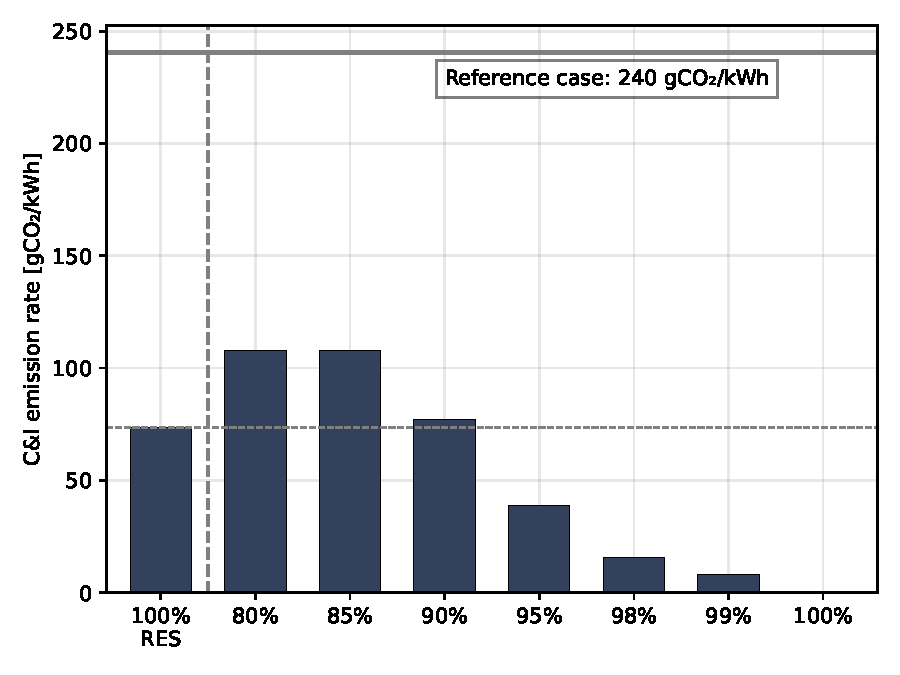
\includegraphics[width=7.5cm]{images/10-2025-DE-p3-ci_emisrate.pdf}
    \end{column}
    \begin{column}{7cm}
      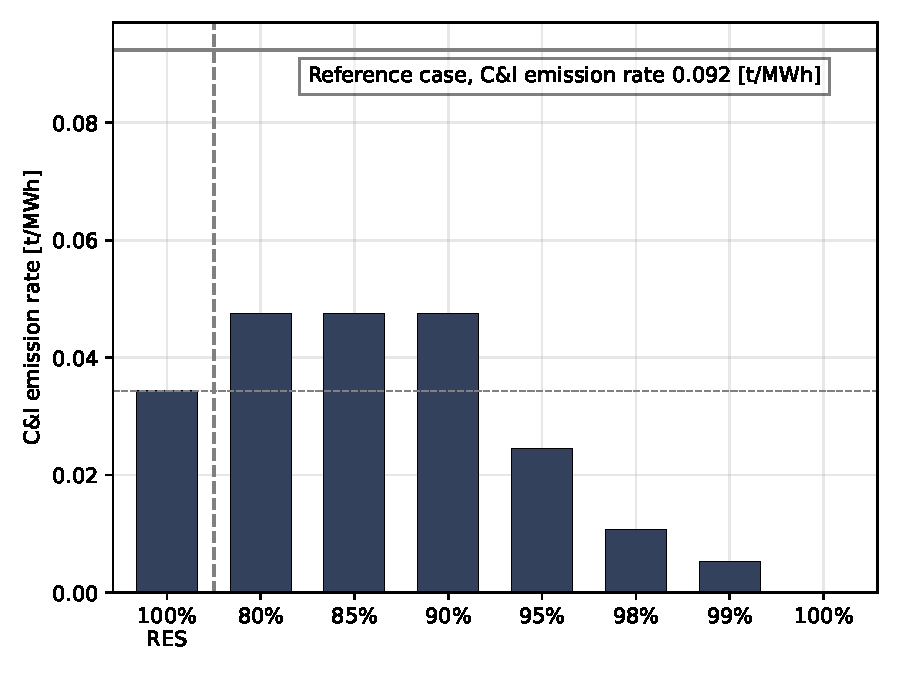
\includegraphics[width=7.5cm]{images/ci_emisrate.pdf}
    \end{column}
  \end{columns}

  Scenario: Germany -- 2025 -- 24/7 CFE with 10\% participation of C\&I sector -- baseload profile -- all costs from \href{https://ens.dk/en/our-services/technology-catalogues}{DEA 2025}. Left: Constrained RES expansion (the Easter Package), Right: unconstrained RES expansion.
\end{frame}


\begin{frame}{Additionality: how we model a background grid 2/2?}
\begin{columns}[t]
	\begin{column}{0.5\textwidth}
		\centering
		\textbf{Two step optimisation} \\
			Clear additionality
			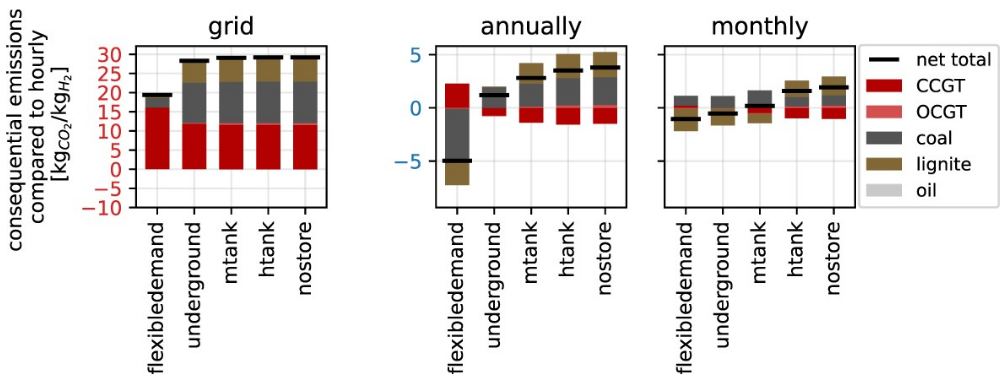
\includegraphics[width=1\linewidth]{images/emissions_twostep_v2}		
	\end{column}
	\begin{column}{0.5\textwidth}
		\centering
		\textbf{One step optimisation} \\
		RES compete for good resources
			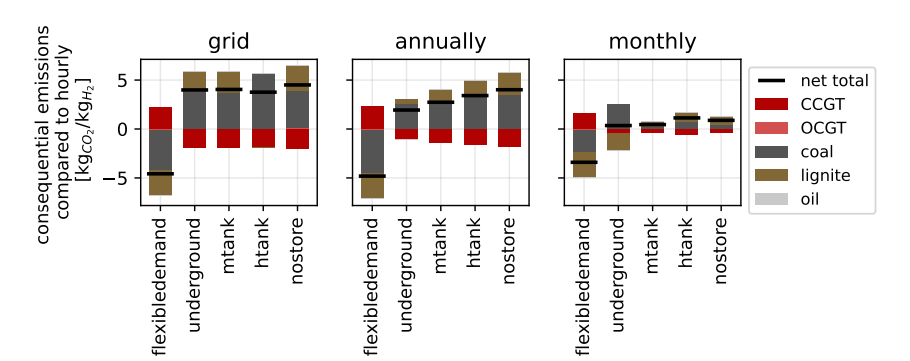
\includegraphics[width=1\linewidth]{images/onestepoptimisation}
	\end{column}
\end{columns}
 There are many studies who analysed the impact on how additionality is modelled in more detail, e.g. \href{https://www.nature.com/articles/s41560-023-01435-0}{Giovanello et al. (2024, Nature Energy), \href{https://papers.ssrn.com/sol3/papers.cfm?abstract_id=4636218}{Langer et al. (2024)}}.
\end{frame}

\section{Take Aways}
\begin{frame}{Take aways}

\begin{columns}
\begin{column}{7cm}
  \begin{enumerate}
    \item Do not take results for granted, try to challenge everything! \\
    \enquote{We must fight our biases to see the solutions} (Auke Hoekstra)
    \item Talk to others in research community, share your concerns! \\
    \enquote{A problem shared is a problem halved} (Old saying)
  \end{enumerate}
\end{column}
\begin{column}{8cm}
  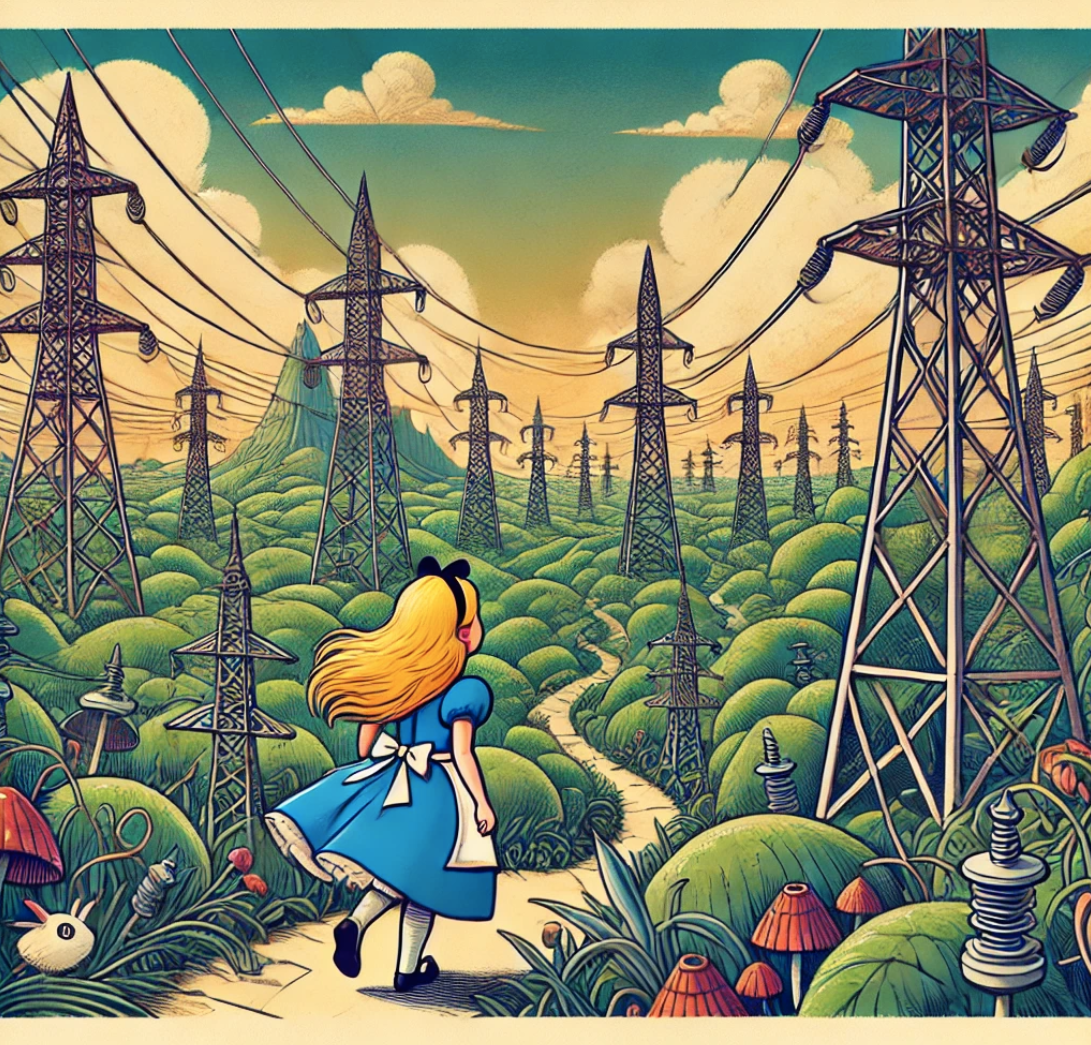
\includegraphics[width=8cm]{images/alice.png}
  \source{ChatGPT4 hallucination, 2024}
\end{column}
\end{columns}


\end{frame}

%----------------------------------------
%----------------------------------------

\begin{frame}\frametitle{\quad}

  {\Large
  \alert{Contacts, Resources, Acknowledgements}
  }

  \vspace{0.1cm}
    
  {\bf References:}
  \hrefc{https://iopscience.iop.org/article/10.1088/1748-9326/ad2239}{Temporal regulation of renewable supply for electrolytic hydrogen (2023)}\\
  {\bf References:} \hrefc{https://irieo.github.io/247cfe.github.io/}{More about the 24/7 CFE research project (2022-2024)}

  {\bf Code:} This work done in a spirit of open and reproducible research: \\
  \faUnlock~code:
  \hrefc{https://github.com/PyPSA/247-cfe}{github.com/PyPSA/247-cfe} \\
  \faUnlock~code: \hrefc{https://zenodo.org/records/8324521}{https://zenodo.org/records/8324521}
  
  \vspace{.1cm}
  {\bf Copyright:} Unless otherwise stated, graphics and text are Copyright \copyright E.Z. and I.R. 2024. \\
  This work is licensed under a \href{https://creativecommons.org/licenses/by/4.0/}{CC BY 4.0}.  {\footnotesize \ccby} 

  \vspace{.1cm}
  {\bf Send an email:} \\
  Dr. Elisabeth Zeyen, e.zeyen@tu-berlin.de\\
  Dr. Iegor Riepin, iegor.riepin@tu-berlin.de \\
  
\end{frame}


%%%%%%%%%%%%%%%%%%%%%%%%%%%%%%%%%%%%%%%%%%%%%%%%%%%%%%
\end{document}
%%%%%%%%%%%%%%%%%%%%%%%%%%%%%%%%%%%%%%%%%%%%%%%%%%%%%%